\chapter{Theory}
\label{Chap:Theory}

This Chapter lays the theoretical groundwork to understand the research presented later in this work, addressing laser wakefield acceleration, radiation production from charged particles and the fundamental processes of radiation reaction and pair production.

Firstly, the equation of motions of charged single particles in electromagnetic fields are derived. This forms the basis for understanding the properties of electrons accelerated in wakefield accelerators, measuring their energy in magnetic spectrometers and calculating the radiation they emit in interaction with electromagnetic fields.

Secondly, the propagation of a laser in a medium and its non-linear evolution, in particular plasmas, are discussed. This paves the way for the third section on laser wakefield acceleration where basic properties like maximum energy and injection mechanisms are introduced.

Then, radiation production from electrons in different scenarios is discussed, starting with radiation in synchrotrons and insertion devices, then drawing the parallel to betatron radiation produced in wakefield acceleration and the radiation emitted in a laser wiggler, namely relativistic inverse Compton scattering (ICS) in moderately (linear ICS) and highly intense laser fields (non-linear ICS).

This leads over to the topic of radiation reaction, the knock-back force a particle experiences when emitting a photon. One suitable tool to investigate radiation reaction is relativistic inverse Compton scattering.

Finally, other fundamental high-field processes as pair production from different mechanisms and future research topics are discussed.

\section{Single particle motion in an EM field}

The Lagrangian for a relativistic particle in an electromagnetic field with the potentials $\Phi$ and $\mathbf{A}$ is given by

\begin{equation}
L(\mathbf{r},\mathbf{v},t) = - mc^2 \gamma^{-1}+q \mathbf{v}\cdot\mathbf{A} - q \Phi,
\end{equation}
where $m$ is the mass of the particle, $\gamma$ the relativistic Lorentz factor and $q$ the charge.

To obtain the equation of motion (EoM) we use the Euler-Lagrange equation

\begin{equation}
\frac{\mathrm{d}}{\mathrm{d}t} \frac{\partial L}{\partial \mathbf{v}} - \frac{\partial L}{\partial \mathbf{r}} = 0.
\end{equation}

Using $\mathbf{A} = \mathbf{A}(\mathbf{r},t)$, $\Phi = \Phi(\mathbf{r},t)$, $\gamma^{-1} = \sqrt{1-(v/c)^2}$ and this becomes

\begin{equation}
\frac{\mathrm{d}}{\mathrm{d}t} \left[\mathbf{p}+q\mathbf{A}\right]-\left[q\nabla\left( \mathbf{A} \cdot \mathbf{v}\right) - q\nabla \Phi \right] = 0,
\label{Theory:Eqns:EoMLorentzRaw}
\end{equation}
where $\mathbf{p} = \gamma m \mathbf{v}$ is the relativistic momentum.

Now using $\frac{\mathrm{d}}{\mathrm{d}t} = \frac{\partial}{\partial t} + \mathbf{v} \cdot \nabla$ and the vector identity $\nabla \left(\mathbf{v}\cdot\mathbf{A}\right) = (\mathbf{v}\cdot\nabla)\mathbf{A} + \mathbf{v}\times(\nabla\times\mathbf{A})$ this becomes:

\begin{equation}
\frac{\mathrm{d}}{\mathrm{d}t}\mathbf{p} = q\left(\mathbf{v} \times \nabla \times \mathbf{A}-\frac{\partial \mathbf{A}}{\partial t} - \nabla \Phi\right).
\label{Theory:Eqns:EoMLorentz}
\end{equation}

With the definitions of the electric field $\mathbf{E}$ and the magnetic field $\mathbf{B}$ in terms of the potentials  $\Phi$ and $\mathbf{A}$
\begin{align}
\mathbf{E} &= -\frac{\partial \mathbf{A}}{\partial t} - \nabla \Phi,\\
\mathbf{B} &= \nabla \times \mathbf{A},
\end{align}

the equation of motion takes the familiar shape of the Lorentz force:

\begin{equation}
\boxed{\frac{\mathrm{d}\mathbf{p}}{\mathrm{d}t} = q \left(\mathbf{E} + \mathbf{v} \times \mathbf{B}\right).}
\end{equation}

\subsection{Electron motion in a homogeneous electric field}

Using the previously derived equation for the Lorentz force we can now consider a first simple example. Consider the motion of a single electron in a homogeneous electric field without presence of a magnetic field, i.e. $\mathbf{B} = \mathbf{0}$. The Lorentz equation simplifies to:

\begin{equation}
\frac{\mathrm{d}\mathbf{p}}{\mathrm{d}t} = q \mathbf{E}.
\end{equation}

If we choose the coordinate system such that  $\mathbf{E} =  (E,0,0)^t = E e_x$, we see that the momentum of the electron is unchanged in the other two directions, $\mathrm{d}p_x/\mathrm{d}t = \mathrm{d}p_y/\mathrm{d}p_y = 0$. In x-direction the electron however feels a constant force $qE$ accelerating it further and further at a linear energy gain.

\subsection{Electron motion in a homogeneous magnetic field}

Consider the motion of a single electron in a homogeneous magnetic field extending over the entire region of interest. The equation for the Lorentz force simplifies with $\mathbf{E} = \mathbf{0}$ to:
\begin{subequations}
\begin{align}
\frac{\mathrm{d}\mathbf{p}}{\mathrm{d}t} &= q \mathbf{v} \times \mathbf{B},\\
\frac{\mathrm{d}\mathbf{p}}{\mathrm{d}t} &= \frac{q}{\gamma m} \mathbf{p} \times \mathbf{B},
\end{align}
\end{subequations}
in terms of the relativistic momentum $\mathbf{p} = \gamma m \mathbf{v}$

Note that in this case the purely magnetic Lorentz force does not do any work. The instantaneous rate of work (power) is $P = \mathbf{F} \cdot \mathbf{v}$, where the force $\mathbf{F}$ is through virtue of the cross product always orthogonal to $\mathbf{v}$ and the dot product vanishes.

We choose the coordinate system such that $\mathbf{B} = (0,0,B)^t = B e_z$. The momentum vector is simply $\mathbf{p} = (p_x,p_y,p_z)^t$.
This then gives us the differential equations:

\begin{subequations}
\begin{align}
\dot{p_x} &= \frac{qB}{\gamma m} p_y,\\
\dot{p_y} &= - \frac{qB}{\gamma m} p_x,\\
\dot{p_z} &= 0,
\end{align}
\end{subequations}
which gives us
\begin{subequations}
\begin{align}
\ddot{p_x}  &= - \left(\frac{qB}{\gamma m}\right)^2 p_x,\\
\ddot{p_y}  &= - \left(\frac{qB}{\gamma m}\right)^2 p_y.
\end{align}
\end{subequations}
This can be solved by a periodic motion of type $p_x(t) = C \sin(\omega t) + D \cos(\omega t)$ with $\omega = qB/\gamma m$. The dotted variables indicate the time derivatives with $\dot{p} = \mathrm{d}p/\mathrm{d}t$ and $\ddot{p}=\mathrm{d}^2p/\mathrm{d}^2t$.

$\mathbf{p_\perp}$ be the momentum vector of the particle perpendicular to the magnetic field lines and $\mathbf{p_\parallel}$ the component parallel to the magnetic field (z). If we assume initial conditions $p_x(t=0) = |\mathbf{p_\perp}| = p_\perp$ and $p_y(t=0)=0$, we obtain for the momenta:
\begin{subequations}
\begin{align}
p_x(t) &= p_\perp \cos(\omega t)\\
p_y(t) &= - p_\perp \sin(\omega t) 
\end{align}
\end{subequations}
The solution for the z-motion is trivial $p_z = p_{z,0}$.

Expressed in terms of the trajectories with initial conditions $x(0) = 0, z(0) = 0, y(0) = p_\perp/qB = r_{L}$, we obtain
\begin{subequations}
\begin{empheq}[box=\widefbox]{align}
x(t) &= r_{L} \sin(\omega t)\\
y(t) &= r_{L} \cos(\omega t)\\
z(t) &= \frac{p_{z,0}}{\gamma m} t
\end{empheq}
\end{subequations}

The radius of the circular motion of the electron is called the Larmor radius $r_L$. It depends on the total momentum in the x-y plane and the magnetic field strength $B$: 
\begin{equation}
r_{L} = |\mathbf{p}_\perp|/eB,
\end{equation}
where $e$ is the charge of the electron and $\mathbf{p}_\perp$ is the component of the momentum vector $\mathbf{p}$ that is perpendicular to the field component of the magnetic field.
\vspace{\baselineskip}

The motion of the electron consists of two decoupled motions: one at the constant, initial velocity parallel to the magnetic field vector in $z$, the second motion is a circular motion in the x-y plane. This is called a cyclotron motion. For now we will ignore the dissipation of energy in form of radiation due to the acceleration of the electron and accept the result that the Lorentz force conserves the total momentum and energy of the particle in this case.

\subsection{Electron motion in a monochromatic plane EM wave}

This derivation is based on Alec Thomas' PhD thesis \cite{ThomasThesis}.

Writing the equation of motion (EoM) in terms of the potentials $\mathbf{A}$ and $\Phi$ as in Equation \eqref{Theory:Eqns:EoMLorentz} on page \pageref{Theory:Eqns:EoMLorentz} gives:

\begin{equation}
\frac{\mathrm{d}}{\mathrm{d}t}\mathbf{p} = q\left(\mathbf{v} \times \nabla \times \mathbf{A}-\frac{\partial \mathbf{A}}{\partial t} - \nabla \Phi\right).
\end{equation}

Now using the convective derivative and the vector identity $\mathbf{v} \cdot \nabla \mathbf{p} = (\nabla \mathbf{p})\cdot\mathbf{v} - \mathbf{v} \times (\nabla\times\mathbf{p})$ again, the total time derivative of the momentum expands to
\begin{equation}
\frac{\mathrm{d}}{\mathrm{d}t}\mathbf{p} = \frac{\partial\mathbf{p}}{\partial t} +(\nabla\mathbf{p})\cdot\mathbf{v} - \mathbf{v}\times(\nabla\times\mathbf{p}).
\end{equation}

With this result the EoM becomes
\begin{align}
\frac{\partial\mathbf{p}}{\partial t} +(\nabla\mathbf{p})\cdot\mathbf{v} - \mathbf{v}\times(\nabla\times\mathbf{p}) &= q\left(\mathbf{v} \times \nabla \times \mathbf{A}-\frac{\partial \mathbf{A}}{\partial t} - \nabla \Phi\right),\nonumber\\
\frac{\partial}{\partial t}\left(\mathbf{p}+q\mathbf{A}\right) +(\nabla\mathbf{p})\cdot\mathbf{v} - \mathbf{v}\times\left(\nabla\times\left(\mathbf{p}+q\mathbf{A}\right)\right) &= - q\nabla \Phi,\nonumber\\
\frac{\partial}{\partial t}\mathbf{u} +(\nabla\mathbf{p})\cdot\mathbf{v} - \mathbf{v}\times\left(\nabla\times\mathbf{u}\right) &= - q\nabla \Phi,
\label{Theory:Eqns:EoMLaserAT}
\end{align}
where in the last step we introduced the canonical momentum $\mathbf{u} = \mathbf{p} + q\mathbf{A}$.

We can express $(\nabla\mathbf{p})\cdot \mathbf{v}$ as follows
\begin{equation}
(\nabla\mathbf{p})\cdot \mathbf{v} = \frac{1}{m\gamma} \nabla (p^2/2) = \frac{1}{m\gamma}\nabla(\gamma^2/2) = m c^2 \nabla \gamma.
\label{Theory:Eqns:nablaDotV}
\end{equation}

Substituting $(\nabla\mathbf{p})\cdot \mathbf{v}$ in Equation \eqref{Theory:Eqns:EoMLaserAT} by the expression in Equation \eqref{Theory:Eqns:nablaDotV}, we obtain
\begin{equation}
\frac{\partial}{\partial t}\mathbf{u} = \mathbf{v}\times\left(\nabla\times\mathbf{u}\right) - \nabla \left(q\Phi + \gamma mc^2\right).
\label{Theory:Eqns:partialtU}
\end{equation}

Taking the curl of this equation results in:
\begin{equation}
\frac{\partial}{\partial t}\nabla\times\mathbf{u} = \nabla\times\left[\mathbf{v}\times\left(\nabla\times\mathbf{u}\right)\right],
\end{equation}
where the second term disappeared as the curl of a gradient is always zero.

This equation shows that if $\nabla \times \mathbf{u}$ is zero initially, it will remain so always. The condition is satisfied, for instance, for a plasma at rest before the laser pulse arrives.

Assuming this condition our Equation \eqref{Theory:Eqns:partialtU} simplifies to
\begin{equation}
\frac{\partial}{\partial t}\mathbf{u} = - \nabla \left(q\Phi + \gamma mc^2\right).
\end{equation}

For a medium close to vacuum or an unperturbed plasma one can assume $\Phi = 0$, resulting in:
\begin{equation}
\frac{\partial}{\partial t}\mathbf{u} =  -\nabla\gamma mc^2.
\end{equation}

In the case of an infinite plane wave the transverse gradient $\nabla_\perp$ is zero.

This means we obtain two separate components:
\begin{subequations}
\begin{align}
\frac{\partial}{\partial t}\mathbf{u}_\perp &= 0,\\
\frac{\partial}{\partial t}\mathbf{u}_\parallel &= \nabla_\parallel \gamma mc^2.
\end{align}
\end{subequations}

From the perpendicular component we see that the transverse canonical momentum is conserved: $\mathbf{p}_\perp + q\mathbf{A} = 0$. If $q = -e$ and $e\mathbf{A}_\perp = \mathbf{a}_\perp$, then $\mathbf{p}_\perp = \mathbf{a}_\perp$. In terms of the Cartesian coordinates, this means $p_x = a_x, p_y = a_y$.

For the parallel spatial component $z$ consider the substitution $z = ct$ for light. Thus, $\partial z = c \partial t$. The parallel-component of the vector potential $\mathbf{A}$ is zero, so $u_\parallel = p_\parallel = p_z$:

\begin{equation}
\frac{\partial}{\partial t}(cp_z - \gamma mc^2) = 0.
\end{equation}

Assuming an unperturbed stationary plasma, the initial conditions are $\gamma(t=0) = 1$ and $p_z(t=0) = 0$. Integrating the previous equation gives:
\begin{equation}
c p_z+ mc^2 = \gamma mc^2.
\end{equation}

Using $E = \gamma m c^2 = \sqrt{mc^2 + (cp_\parallel)^2 + (cp_\perp)^2}$ and substituting, one obtains an expression for $p_\parallel = p_z$:

\begin{equation}
p_z = \frac{1}{2} mc a^2,
\end{equation}
where $a^2 = p^2_\perp$.

We now have
\begin{subequations}
\begin{align}
p_x &= mc a_x,\\
p_y &= mc a_y,\\
p_z &= \frac{1}{2} mc a^2.
\end{align}
\end{subequations}

Using $\mathbf{p} = \gamma m \mathbf{v}$ this can be written as:
\begin{subequations}
\begin{align}
\frac{\gamma}{c} \frac{\mathrm{d}x}{\mathrm{d}t} &= a_x,\\
\frac{\gamma}{c} \frac{\mathrm{d}y}{\mathrm{d}t} &= a_y,\\
\frac{\gamma}{c} \frac{\mathrm{d}z}{\mathrm{d}t} &= \frac{a^2}{2}.
\end{align}
\end{subequations}

Changing from $t$ to proper time $\tau$, we transform via $\mathrm{d}\tau = \gamma^{-1}\mathrm{d}t$, simply giving the equation of motions in term of $\tau$:
\begin{subequations}
\begin{align}
\frac{1}{c}\frac{\mathrm{d}x}{\mathrm{d}\tau} &= a_x,\\
\frac{1}{c}\frac{\mathrm{d}y}{\mathrm{d}\tau} &= a_y,\\
\frac{1}{c}\frac{\mathrm{d}z}{\mathrm{d}\tau} &= \frac{a^2}{2}.
\end{align}
\end{subequations}

Let us assume a laser field with linear polarisation in $x$, described by the vector potential
\begin{equation}
\mathbf{a} = a_0 \cos(kz - \omega t)\mathbf{e}_x = a_0 \cos(\xi)\mathbf{e}_x,
\end{equation}
where $\mathbf{e}_x$ is the unit vector in the x-coordinate, $\xi = kz - \omega t$ the waveframe coordinate and $k = \omega/c$ the wave number. 

\begin{figure}[h]
\centering
	\includegraphics[width=0.49\columnwidth]{figeight_lab.pdf}
	\includegraphics[width=0.49\columnwidth]{figeight_drift.pdf}
\caption[Electron motion in an infinite, linearly polarised, plane EM wave.]{Electron motion in an infinite, linearly polarised, plane EM wave in the lab frame (left), with the wavenumber $k = \omega/c$. On the right the figure-of-eight motion in the drift frame.}
\label{Theory:Figs:FigureOfEight}
\end{figure}

Using this explicit vector potential:
\begin{subequations}
\begin{align}
\frac{\gamma}{c}\frac{\mathrm{d}x}{\mathrm{d}t} &= a_0 \cos \xi,\\
\frac{\gamma}{c}\frac{\mathrm{d}y}{\mathrm{d}t} &= 0,\\
\frac{\gamma}{c}\frac{\mathrm{d}z}{\mathrm{d}t} &= \frac{1}{2} a^2_0 \cos^2 \xi.
\end{align}
\end{subequations}

and integrating the equation of motions, results in:
\begin{subequations}
\begin{align}
x(\xi) &= \frac{a_0}{k}\sin(\xi),\\
y(\xi) &= 0,\\
z(\xi) &= \frac{a^2_0}{4k}\left(\xi + \frac{1}{2}\sin(2\xi)\right),
\end{align}
\end{subequations}
where we chose the initial conditions $x(0)=y(0)=z(0)=0$  and used $\mathrm{d}\xi/\mathrm{d}t = \omega/\gamma$.

The electron is performing a periodic oscillation around the z-axis, whilst the motion in the z-axis is composed of a constant drift and another oscillation (see figure \ref{Theory:Figs:FigureOfEight} (left)). This is commonly referred to as the `figure-of-eight' motion, which becomes more evident in the drift frame (see figure \ref{Theory:Figs:FigureOfEight} (right)). For $a_0 \leq 1$ the motion in z is suppressed and the motion of the electron is dominated by the transverse oscillation. For $a_0 \gg 1$, the motion is predominantly longitudinal.



\subsection{Electron in a cylindrically symmetric electric field}

The previously discussed case of a particle in a homogeneous magnetic field corresponds to the motion in a magnetic electron spectrometer or the deflection of charged particles in a circular accelerator.
We will now discuss the motion of an electron in a cylindrically symmetric electric field. This resembles the case of an electron in a plasma channel.

Assume a relativistic electron moving in the longitudinal direction and an electric field that is cylindrically symmetric around the propagation axis.

As previously we will use a Lagrangian. We ignore any vector potential contributions and only use a scalar potential.

The Lagrangian of this scenario is described by

\begin{equation}
L(\mathbf{r},\mathbf{v},t) = - m_e c^2 \gamma^{-1} - q \Phi
\end{equation}
where $\Phi$ is the scalar potential describing the electrostatic field of the channel.

The scalar potential is the solution matching the radially/cylindrically symmetric Poisson equation

\begin{equation}
\frac{1}{r} \frac{\partial}{\partial r} \left(r \frac{\partial \phi}{\partial r}\right) = \frac{- e (n_0 - n_e)}{\epsilon_0}
\end{equation}

The solution is 
\begin{equation}
\phi = -\frac{(n_0 - n_e) e r^2}{4 \epsilon_0}
\end{equation}

In the extreme case of a completely evacuated channel, $n_e \rightarrow 0$, $\phi = -n_0 er^2/(4\epsilon_0)$.

As before $\mathbf{E} = - \nabla \phi$ and in this case $E_r = - \partial_r \phi$.

The equation of motion for the radial component is then

\begin{equation}
\frac{d}{dt} \mathbf{p} = - \frac{e^2 n_0}{2 \epsilon_0} r
\end{equation}

Assume there is no axial acceleration field, and the radial component of the velocity is small compared to $c$ and the longitudinal component be close to $c$: $\dot{\gamma}$ is then close to zero. $\mathbf{p} = \gamma m_e \mathbf{\dot{r}}$

The equation then takes the shape of a harmonic oscillator

\begin{equation}
\ddot{r} = - \frac{e^2 n_0}{2\epsilon_0 m_e \gamma} r = - \omega_\beta^2 r
\end{equation}

with a frequency we will call the betatron frequency $\omega_\beta$.


\EliasComm{Treat second-order motion and find it follows a figure-of-eight motion!}

\subsection{Electron in a cylindrically symmetric electric field with axial field}


Now in addition to the previous case we will add an axial field in the longitudinal (direction of electron propagation). This comes closer to the reality of a laser wakefield accelerator where electrons experience focusing and accelerating fields at the same time.
The electric field component shall now be $E_z$, with $z$ being the longitudinal axis.
This gives us an extra term $\frac{\partial \phi}{\partial z} = - E_z$.

The Euler-Lagrangian now has two equations of motions.

Firstly, as before
\begin{equation}
\frac{d}{dt} (\gamma m_e \dot{r}) = \frac{\partial }{\partial r} L = -\frac{e^2 n_0}{2\epsilon_0} r
\end{equation}

Secondly the z-component
\begin{equation}
\frac{d}{dt} (\gamma m_e \dot{z}) = \frac{\partial }{\partial z} L = e E_z = const.
\end{equation}

This time the change in momentum in time is not negligible and we have to expand the brackets.

Radial component:
\begin{equation}
\dot{\gamma}m_e \dot{r} + \gamma m_e \ddot{r} = - \frac{e^2 n_0}{2 \epsilon_0} r
\end{equation}

Axial component is equal to a constant so simply by integrating
\begin{equation}
\gamma m_e \dot{z} = - e E_z t + const.
\end{equation}

If we assume that the electron is highly relativistic $\dot{z} \rightarrow c$, so $\dot{\gamma} = eE_z/m_e c$ and

\begin{equation}
\gamma \beta_z \approx \gamma = - \frac{e E_z t}{m_e c} + \gamma_0 \beta_0,
\end{equation}

where $\gamma_0 \beta_0$ are the initial conditions.

\begin{figure}
\centering
\includegraphics[width=.5\columnwidth]{betatron_traj.png}
\caption{Particle trajectory of an electron using the initial conditions INSERT HERE, an accelerating gradient of NUMBER and XXXXX. Used same numbers and notations as Jon but somehow the plot scales differently. REPLACE.}
\end{figure}


Based on Jon Wood's thesis \cite{WoodThesis}
Combining both results and keeping the same assumptions:

\begin{equation}
eE_z \dot{r} + (eE_z t + \gamma_0 \beta_0 m_e c) \ddot{r} = - \frac{e^2 n_0 c}{2 \epsilon_0} r
\end{equation}

Abbreviating some terms....

\begin{equation}
(At + B) \ddot{r} + A \dot{r} + C r = 0
\end{equation}

\begin{equation}
r(t) = \frac{\pi \sqrt{CB}}{A} r_{\beta 0} \left[ J_1 \left( 2 \sqrt{CB}/A \right) Y_0 \left(2 \sqrt{C (B+At)}/A\right) - Y_1 \left(2\sqrt{CB}/A\right)J_0\left(2\sqrt{C(B+At)}/A\right)\right]
\end{equation}
with the initial conditions $r(t=0) = r_{\beta 0}$ and $\dot{r}(t=0) = 0$. 
\vspace{\baselineskip}

The oscillations quickly lose amplitude and frequency to a settled value as the electron gains momentum and hence inertia.


\subsection{Electron in a periodically alternating magnetic field}

This is the scenario of an electron in an insertion device. The electron follows a figure-of-eight motion.

\subsection{Ponderomotive Force}

In laser wakefield acceleration (LWFA) a high intensity laser pulse propagates through an underdense plasma, expels electrons in its way and drives a wave. The driving force is the so-called ponderomotive force which is proportional to the gradient of the laser intensity. 

The following relativistic derivation of the ponderomotive force is based on Alec Thomas' PhD thesis \cite{ThomasThesis}.

We start with the Euler-Lagrange equations after plugging in the Lagrangian in terms of the potentials $\mathbf{A}$ and $\Phi$ as given as intermediate step in equation \eqref{Theory:Eqns:EoMLorentzRaw} on page \pageref{Theory:Eqns:EoMLorentzRaw}:

\begin{equation}
\frac{\mathrm{d}}{\mathrm{d}t} \left[\mathbf{p}+q\mathbf{A}\right]-\left[q\nabla\left( \mathbf{A} \cdot \mathbf{v}\right) - q\nabla \Phi \right] = 0.
\end{equation}

This can be written in terms of the normalised quantities
\begin{align}
\mathbf{a} &= -q \mathbf{A}/m_e c,\nonumber\\
\phi &= -q\phi/mc^2,\nonumber\\
\mathbf{v} &\rightarrow \beta = \mathbf{v}/c,\nonumber\\
\mathbf{p} &\rightarrow \mathbf{p}/m c,
\end{align}

resulting in

\begin{equation}
\frac{\mathrm{d}}{\mathrm{d}t} \left[\mathbf{p}-\mathbf{a}\right] - \left(c\nabla \mathbf{a}\right) - c \nabla \phi = 0.
\end{equation}

Using the canonical momentum $\mathbf{u} = \mathbf{p} - \mathbf{a}$ the time derivative can now be re-written and we can also substitute $\mathbf{v} = \mathbf{p}/\gamma = (\mathbf{u}+\mathbf{a})/\gamma$:

\begin{align}
\frac{\mathrm{d}}{\mathrm{d}t}\mathbf{u} &= c\nabla\phi - (c\nabla\mathbf{a})\cdot\frac{(\mathbf{u}+\mathbf{a})}{\gamma},\nonumber\\
\frac{\mathrm{d}}{\mathrm{d}t}\mathbf{u} &= c\nabla\phi - \frac{1}{\gamma} c \nabla \frac{\mathbf{a}^2}{2}-c\nabla\mathbf{a}\cdot\frac{\mathbf{u}}{\gamma}.
\end{align}

In the scenario of an electromagnetic pulse at high frequency $\omega$ of long pulse duration $\tau \gg 1/\omega$ and sufficiently large spot size $w \gg 1/|k|$ in terms of the fast oscillations, fast and slow dynamics can be treated separately.

When averaging over the time of a period $T = 2\pi/\omega$, the terms of linear order $\mathbf{a}$ and the potential $\phi$ amount to zero:
\begin{equation}
\boxed{\left\langle\frac{\mathrm{d}}{\mathrm{d}t}\mathbf{u}\right\rangle \sim -\left\langle\frac{1}{\gamma}c\nabla\frac{\mathbf{a}^2}{2}\right\rangle,}
\end{equation}
which is the ponderomotive force $\mathbf{F}_p$ on on a single electron. Since $\mathbf{F}_p \sim \nabla \left\langle\mathbf{a}^2\right\rangle$, this implies $\mathbf{F}_p \sim \nabla \left\langle I\right\rangle$, i.e. the ponderomotive force pushes electrons away from regions of high intensity and is hence a suitable force to drive LWFA.


\iffalse
As the force is essential for the understanding of LWFA it will be derived in the following.

A derivation (Kruer), THIS SECTION NEEDS WORK AS IT IS SO FAR ALMOST 1:1 TAKEN FROM KRUER


HERE A COMMENT WHAT ASSUMED TO TAKE E(x) without the -kx term, as it is a wave actually....

Consider response of a homogeneous plasma to a high frequency field with spatially dependent amplitude $E = E(x) \sin(\omega t)$. We assume $\omega$ is around the electron plasma frequency which in turn is much larger than the frequency of the ion species. The electrons are treated as a fluid and the electron pressure is neglected.

The force equation:
\begin{equation}
\frac{\partial u_e}{\partial t} + u_e \cdot \nabla u_e = - \frac{e}{m} E(x) \sin(\omega t).
\end{equation}

To lowest order $|E|$, $u_e = u^h$ (what is h?)

\begin{equation}
\frac{\partial u^h}{\partial t} = -\frac{e}{m} E(x) \sin(\omega t),\\
u^h = \frac{eE}{m\omega} \cos(\omega t).
\end{equation}

The electrons are oscillating in the electric field. Averaging over the force equation over these oscillations:
\begin{equation}
m \frac{\partial u^s}{\partial t} = -e E^s - m \langle u^h \cdot \nabla u^h \rangle_t,
\end{equation}
where the brackets with index t denote the time average over the high frequency oscillations and $u^s$ is the time average of $u_e$.

Now substituting for $u^h$ from our previous result this gives 

\begin{equation}
m \frac{\partial u^s}{\partial t} = - e E^s - \frac{1}{4} \frac{e^2}{m \omega^2} \nabla E^2(x).
\end{equation}

In addition to the linear term we observe a force that pushes away electrons from regions of high field pressure. The ponderomotive force is proportional to the gradient of the electric field pressure:
\begin{equation}
F_p = - \frac{e^2}{4 m \omega} \nabla E^2 (x)
\end{equation}

When considering this in the relativistic regime, for instance in \cite{Quesnel1998}

in terms of the normalised vector potential
\begin{equation}
F_p = - \frac{1}{2} m_e c^2 \frac{1}{|\gamma|}\nabla \langle a^2 \rangle.
\end{equation}


ANOTHER DERIVATION HERE BASED ON ALEC THOMAS

USE ONE BIT TO EXPLAIN LASER WAKEFIELD ACCELERATION, TAKE THE SECOND TERM TO GO FOR PWFA (PONDEROMOTIVE FORCE MISSING)

\fi



\section{Laser Propagation in an Underdense Medium}

\subsection{Plasma Properties}

A plasma is an on average charge-neutral medium that consists of charged particles, in the context of wakefield acceleration ions and free electrons. This property is called quasi-neutrality and can mathematically be expressed as
\begin{equation}
-e n_e + Z e n_i \approx 0,
\end{equation}
where $e$ is the fundamental charge, $n_e$ the electron number density, $n_i$ the ion number density and $Z$ the charge number of the ions.
Whilst this balance might locally not be true at every moment in time, the mobility of the charges lead to shielding at length scales larger than the Debye length $\lambda_D$:
\begin{equation}
\lambda_D = \left(\frac{\epsilon_0 k_B T_e}{n_e e^2}\right)^{1/2},
\end{equation}
where $\epsilon_0$ is the dielectric constant, $k_B$ the Boltzmann constant and $T_e$ the electron temperature. 

The formation of Debye-spheres is an example of a collective response of the plasma to a small perturbation. In a plasma particles can act together on macroscopic scales through long range electromagnetic forces to form instabilities and waves. Even small imbalances can stimulate a significant response of the medium. This means that even though plasmas can be modelled as fluids and simulated using hydrodynamic codes, introducing electromagnetic forces will give rise to more complex and exotic phenomena than in fluids dominated by gravitational forces.

\subsection{Plasma Formation}

In the context of this work, the process of forming a plasma is usually set equal to ionising a medium consisting of neutral atoms or molecules by applying an electric field in shape of an intense laser pulse. The resulting collection of unbound electrons and ions is a plasma. After a certain time the electrons will return to the ionic cores of the atoms and back again to a bound energy state emitting any excess energy in form of radiation in the process. This is called recombination and the emitted radiation recombination light.

There are different mechanisms through which an oscillating laser field ionises a gas. In single and multi-photon ionisation \cite{Keldysh1965_ION}, one electron is excited by absorbing one or multiple photons, respectively, before decaying to its original ground state. Another mechanism relies on the collision of electrons and atoms \cite{Latypov1964_ION}. The electric field of the laser can also distort the Coulomb potential of the atom, resulting in a finite probability for electrons to tunnel into the continuum \cite{Perelomov1966_ION}.

The dominant ionisation mechanism is indicated by the Keldysh parameter $\gamma_K$ considering the strength of the electric field $E$ relative to the binding potential $V$ and the frequency of the oscillating field $\omega$:
\begin{equation}
\gamma_K = \omega \frac{\sqrt{2 m_e V}}{eE}.
\end{equation}
At $\gamma_K \gg 1$ multiphoton ionisation dominates, whereas for small $\gamma_K < 0.5$ tunnel ionization is expected to be important. If the electric field is larger than the binding Coulomb potential, the atom is immediately ionised: this is called barrier-suppression ionisation \cite{Reiss1970_ION}.

\iffalse
\begin{figure}
\centering
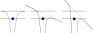
\includegraphics[width=0.9\columnwidth]{ionisation_sketch.png}
\caption{Sketch of ionisation mechanisms.}
\end{figure}
\fi

In the simple example of a hydrogen-like atom in an external electric field $E$, the potential $V$ at a distance $r$ from the core is given by
\begin{equation}
V(r) = -\frac{Ze^2}{4\pi\epsilon_0 r} - eEr,
\end{equation}
where the position of the maximum potential is given by $r_{max} = (Ze/4\pi\epsilon E)^{1/2}$. 

Hence the electric field required for complete barrier suppression of an ionisation potential $V_e$ amounts to

\begin{equation}
E = \frac{\pi \epsilon_0 V^2_e}{Ze^3} \approx 173.6 \times \left(\frac{V_e}{eV}\right)^2 \frac{1}{Z} \, \mathrm{MV/m},
\end{equation} 

or in terms of intensity using $I = \frac{c\epsilon_0}{2}|E|^2$ in (near) vacuum:

\begin{equation}
I = \frac{c\epsilon_0^3 \pi^2 V^4_e}{2e^6 Z^2} \approx 4 \times 10^{9} \left(\frac{V_e}{eV}\right)^4\frac{1}{Z^2} \,\mathrm{W/cm^2}.
\end{equation}

For hydrogen with $V_e = 13.6\,\mathrm{eV}$ the lower bound intensity required for barrier-suppression ionisation amounts to $1.37 \times 10^{14} \,\mathrm{W/cm^2}$, for helium with $Z=2$ and $V_e = 54.4\,\mathrm{eV}$ the equation gives $I = 8.76\times10^{15}\,\mathrm{W/cm^2}$.
The laser intensities in LWFA experiments routinely reach peak intensities above $10^{18}\,\mathrm{W/cm^2}$. Hence, one can safely assume that ionisation effects are negligible for low-$Z$ gases. Higher-$Z$ gases like nitrogen are not as easily fully ionised: in hydrogen-like nitrogen the last electron is bound by a potential of $V_e = 667\,\mathrm{eV}$ at $Z = 7$, which translates in intensities required in excess of $10^{19}\,\mathrm{W/cm^2}$. Even very intense laser pulses might struggle to fully ionise a nitrogen gas at all and one can not assume any longer that a fully ionised plasma is in place when the main part of the laser pulse arrives. The gas might then reach higher degrees of ionisation only at peak fields of the laser either through full barrier suppression or by triggering an increased tunnelling rate: this is taken advantage of in an injection method for wakefields called `ionisation injection' \cite{McGuffey2010_ION,Pak2010_ION}. Partially ionised plasmas are more complex systems as one has to consider, for instance, ionisation effects, absorption of X-rays, weaker fields, dampening of particles, scattering and so on.

\iffalse
\begin{table}
\centering
\begin{tabular}{l|r|l}
Transition & $V_e [\mathrm{eV}]$ & $I_L [\mathrm{W\,cm^{-2}}]$\\ \hline \hline
$H \rightarrow H^+$ & $13.6$ & $1.4 \times 10^{14}$ \\ \hline
$He \rightarrow He^+$ & $24.6$ & $1.5 \times 10^{15}$\\
$He^+ \rightarrow He^{2+}$ & $54.4$ & $8.8 \times 10^{15}$\\ \hline
$N \rightarrow N^+$ & $14.5$ & $1.8 \times 10^{14}$\\
$N^+ \rightarrow N^{2+} $ & $29.6$ & $7.7 \times 10^{14}$\\
$N^{2+} \rightarrow N^{3+} $ & $47.4$ & $2.2 \times 10^{15}$\\
$N^{3+} \rightarrow N^{4+} $ & $77.5$ & $9.0 \times 10^{15}$\\
$N^{4+} \rightarrow N^{5+} $ & $97.9$ & $1.5 \times 10^{16}$\\
$N^{5+} \rightarrow N^{6+} $ & $552.1$ & $1.0 \times 10^{19}$\\
$N^{6+} \rightarrow N^{7+} $ & $667.0$ & $1.6 \times 10^{19}$
\end{tabular}
\caption{Binding energies and required laser intensities for barrier suppression ionisation. REF NIST ASD. Using equation XX with Z being $Z_{eff}=\,$final state ionisation level of ions.}
% @Misc{NIST_ASD,
%author = {A.~Kramida and {Yu.~Ralchenko} and
%J.~Reader and {and NIST ASD Team}},
%HOWPUBLISHED = {{NIST Atomic Spectra Database
%(ver. 5.6.1), [Online]. Available:
%{\tt{https://physics.nist.gov/asd}} [2019, March 25].
%National Institute of Standards and Technology,
%Gaithersburg, MD.}},
%year = {2018},
%}
\end{table}
\fi

\subsection{The Plasma Frequency}

The plasma frequency $\omega_p$ is the natural frequency at which electrons will oscillate in a plasma when displaced. It constitutes the typical time scale and the corresponding plasma wavelength $\lambda_p$ the typical length scale of the medium.
\vspace{\baselineskip}

Assume a uniform and neutral plasma, i.e. $n_e = Z n_i = n_{e0}$, where $n_e$ is the electron number density, $Z$ the charge number of the ions, $n_i$ the ion number density, and the initial electric field be $\mathbf{E} = \mathbf{0}$.
Now consider displacing a slab of charge in an arbitrary direction defining an axis that we will call X.

Starting with Gauss' Law:
\begin{equation}
\nabla \cdot \mathbf{E} = \frac{\rho}{\epsilon_0} = \frac{\partial E_x}{\partial x},
\end{equation}
where we used that the displacement is only along $x$, simplifying the Nabla operator to a spatial derivative in $x$.

We assume a uniform plasma so the charge density is a constant $\rho = e n_{e0}$. Integrating the previous equation then gives a constant factor times the displacement X:
\begin{align}
E_x = \frac{1}{\epsilon_0} \int^x_0 \rho (x') dx' + E_x(0) &= \frac{e n_{e0}}{\epsilon_0} X,\nonumber\\
E &= \frac{e n_{e0}}{\epsilon_0} X.
\end{align}

If we now consider a force based on this field, we immediately see that this is equivalent to the equation of motion of a harmonic oscillator: 

\begin{equation}
m_e \frac{\mathrm{d}^2 X}{\mathrm{d}t^2} = - \frac{e^2 n_e}{\epsilon_0} X = - \omega^2_p X,
\end{equation}

with the (plasma) frequency
\begin{equation}
\boxed{\omega_p = \sqrt{\frac{n_{e0} e^2}{\epsilon_0 m_e}},}
\end{equation}

and the corresponding wavelength $\lambda_p = 2 \pi c/\omega_p$.

\begin{figure}
\centering
\includegraphics[width=.5\columnwidth]{omegap_lambdap_density.pdf}
\caption{Plasma frequency (blue) and wavelength (red) as function of plasma density.}
\end{figure}

A typical regime wakefield accelerators in the context of this work operate in is at an electron density of around $10^{18}-10^{19}\,\mathrm{cm^{-3}}$. This corresponds to a plasma frequency of $(5.6 - 17.7) \times 10^{13} \,\mathrm{Hz}$ or a plasma wavelength of $\lambda_p \approx 33-10\,\mathrm{\mu m}$.

\subsection{Laser Propagation in Vacuum}

An electromagnetic wave of arbitrary shape $u$ has to satisfy Maxwell's equations and hence also the wave equation \cite{Jackson}

\begin{equation}
\left(\nabla^2 - \frac{1}{v^2}\frac{\partial^2}{\partial t^2} \right) u= 0,
\end{equation}
where $v = c/\sqrt{\mu \epsilon}$ and in vacuum $v = c$.

In the case of waves with an electric field $\mathbf{E} = \mathbf{E}(\mathbf{r},t) = \mathbf{u}(\mathbf{r}) v(t)$, where the spatial and temporal dependencies can be separated, the components solve two separate differential equations 
\begin{align}
\left(\nabla^2 + k^2\right) \mathbf{u} &= 0,\\
\left(\frac{\partial^2}{\partial t^2} + k^2\right) v &= 0,
\end{align}
where $k = \sqrt{\mu \epsilon} \omega/c$. The spatial component is called the Helmholtz equation.

For an an electric field $\mathbf{E} = \mathbf{E_0}(r,z) e^{i(kz-\omega t)}$ with cylindrical symmetry in the paraxial approximation $|k \mathbf{E}_0| \gg |\partial_z \mathbf{E}_0|$ the Helmholtz equation takes the form
\begin{equation}
\left(\frac{\partial^2}{\partial r^2} + \frac{1}{r}\frac{\partial}{\partial r}- 2ik \frac{\partial}{\partial z}\right) \mathbf{E}_0 = 0.
\end{equation}

For an in x-direction linearly-polarised electric field moving in $z$ the solution takes the form
\begin{equation}
\mathbf{E}(r,z,t) = E_0 \frac{w_0}{w(z)} \exp\left(-\frac{r^2}{w(z)^2}\right) \exp\left[-i(kz-\omega t)-i k\frac{r^2}{2 R(z)} + i \zeta (z)\right]\mathbf{\hat{x}}.
\end{equation}
This family of solutions is referred to as Gaussian modes and the physical properties of the beam are captured in the different parameters of the wave function. The function $\mathbf{E}$ describes a beam converging from $z < 0$ at a size $w(z)$ onto a minimum at $z = 0$ achieving the highest energy field strengths before diverging again for $z > 0$.
\vspace{\baselineskip}

$w(z)$ is the waist size of the Gaussian beam at position $z$ and indicates the transverse size of the beam when the intensity drops to $1/e^2$ of its maximum:
\begin{equation}
w(z) = w_0 \sqrt{1+ \left(\frac{z}{z_R}\right)^2},
\end{equation}
where $w_0$ is the waist size at focus $z=0$ and $z_R$ the Rayleigh length defined as 
\begin{equation}
z_R = \frac{\pi w^2_0}{\lambda},
\end{equation}
and is the distance over which a Gaussian beam expands from $w_0$ to $\sqrt{2}w_0$ and is hence an indicator for how quickly a beam diverges or in other words over which distance it maintains an intensity close to its maximum.

Assuming the beam is a Gaussian in both time and space the intensity is given by
\begin{equation}
I(r,t) = I_0 \exp\left( -\frac{2 r^2}{w^2_0}\right) \exp\left(-\frac{2 t^2}{\tau^2}\right),
\end{equation}
\EliasComm{This equation is from Jon's thesis \cite{WoodThesis}, but I am missing the z component here. Has to be reviewed. This is at focus.}

$R(z)$ is the radius of curvature of the wavefront
\begin{equation}
R(z) = z \left[1+\left(\frac{z_R}{z}\right)^2\right].
\end{equation}
The wavefront is strongly curved around the focus $z < z_R$ and slowly flattens out at $z \gg z_R$. The difference of in radii of curvature for beams with different Rayleigh length can be used in spatial interferometry applied in the context of synchronising two laser pulses in time.

$\zeta$ is called the Guoy phase and is an additional phase term that changes signs once the Gaussian mode passes through its focus.

When focusing down a beam with an optic, for instance an off-axis parabola or spherical mirror, the ratio of the focal length $f$ and the beam diameter $d$ is a useful quantity as it indicates how tightly a beam is focussed. It is called the f-number $f_\# = f/d$ and is in shorthand typically written as $f/2$ for $f_\# = 2$, $f/40$ for $f_\# = 40$ and so on.
Expressing some of the previous quantities in terms of the f-number 
\begin{equation}
w_0 = \frac{2 \sqrt{2}}{\pi} \lambda f_\# \approx 0.9 \lambda f_\#
\end{equation}
and the distance over which laser stays intense
\begin{equation}
z_R = \frac{\pi w^2_0}{\lambda} \approx 2.5 \lambda f^2_\#.
\end{equation}

In the context of this work a Ti:Sa laser at $\lambda = 800\,\mathrm{nm}$ and these two f-numbers are relevant:

\begin{align*}
f/2: &w_0 = 1.4\, \mathrm{\mu m}; z_R = 8.1 \,\mathrm{\mu m}\\
f/40: &w_0 = 28.8\, \mathrm{\mu m}; z_R = 3200\, \mathrm{\mu m}\\
\end{align*}


However, real laser beams in experiments are typically not Gaussian but mostly flat-top beams. In addition, changes in the wave front, curvature profile, spatio-temporal couplings and so on consist further deviations from an ideal beam. These are commonly expressed in terms of the parameter $M^2$, with the minimum spot size being the ideal diffraction-limited spot size times $M^2$.


\subsection{Laser Propagation in Plasma}

Consider a quasi-neutral plasma (charge density $\rho \approx 0$) with a current density $\mathbf{j} = -e n_e \mathbf{v}$, depending on the velocity $\mathbf{v}$ of the electrons in the plasma and the electron density $n_e$. The wave equation for the electric field $\mathbf{E}$ becomes

\begin{equation}
\nabla^2 \mathbf{E} = - \mu e n_e \frac{\partial \mathbf{v}}{\partial t} + \frac{1}{c^2} \frac{\partial^2 \mathbf{E}}{\partial t^2}.
\end{equation}

The acceleration of the electrons is due to the electric field of the wave, i.e. $\partial \mathbf{v}/\partial t = -e\mathbf{E}/m_e$. Now using the solution for a plane wave with $\mathbf{E} = \mathbf{E_0} \exp \left[i (\mathbf{k}\cdot\mathbf{r} - \omega t) \right]$ the dispersion relation is given by $\omega = c k \left[1-\left(\frac{\omega_p}{\omega}\right)^2\right]^{-1/2}$, and hence the group velocity $v_g$ and the phase velocity $v_p$ are given by:

\begin{align}
v_p &= \frac{\omega}{k} = \frac{c}{\sqrt{1-\left(\frac{\omega_p}{\omega}\right)^2}},\\
v_g &= \frac{\partial\omega_L}{\partial k} = c \sqrt{1-\left(\frac{\omega_p}{\omega}\right)^2},
\end{align}
where $\omega$ is the frequency of the electromagnetic wave.

At $\omega \ll \omega_p$ this the expression can be approximated by
\begin{align}
v_p &= \frac{\omega}{k} \approx c \left(1+ \frac{1}{2}\frac{\omega^2_p}{\omega^2}\right),\\
v_g &= \frac{\partial\omega}{\partial k} \approx c \left(1 - \frac{1}{2}\frac{\omega^2_p}{\omega^2}\right).
\end{align}


\begin{figure}
\centering
\includegraphics[width= 0.5\columnwidth ]{GroupVelocity_density.pdf}\includegraphics[width=0.5\columnwidth]{critical_density.pdf}
\caption[Group velocity at different densities and critical densities for different laser wavelengths.]{Left: Group velocity at different densities for photons of wavelength $\lambda = 0.8\,\mathrm{mu}$ (blue) and $10\,\mathrm{\mu}$ (orange) in units of the vacuum speed of light (indicated in green). The red dotted line shows the density at which the group velocity reaches zero, called the critical density. Right: Critical density for wavelengths up to $2 \mu m$ (blue). The critical density corresponding to a central wavelength of $0.8 \mu m$, as for the commonly used titanium-doped sapphire (Ti:Sa) lasers, is marked in red on the graph. The region above the critical density (blue line) is called overdense, below underdense.}
\end{figure}

The group velocity reaches zero for $\omega_p = \omega$, where $\omega_p$ is the plasma frequency, derived in the previous section and given by $\omega_p = (n_e e^2/\epsilon_0 m_e)^{1/2}$. Solving this for the density, we obtain a relation for the critical density:

\begin{equation}
\boxed{n_c = \frac{m_e \epsilon_0 \omega^2}{e^2},}
\end{equation}
which only depends on the frequency of the incident electromagnetic wave, and so we can write the refractive index $\eta = c/v_p$ in terms of the electron density $n_e$ and the critical density $n_c$:

\begin{equation}
\eta = \sqrt{1-\left(\frac{\omega_p}{\omega}\right)^2} = \sqrt{1-\frac{n_e}{n_c}}.
\end{equation}

For $n_e > n_c$, called an `overdense plasma', the refractive index is imaginary and the wave becomes evanescent in the medium. This means a wave can only enter the material up to a skin depth before being reflected again.
A plasma with a density $n_e < n_c$ is transparent and called `underdense'. LWFA requires the laser pulse to propagate through the plasma to drive the wave and hence targets used are typically operating at densities of only a fraction of $n_c$, whilst many ion acceleration mechanisms are based on overdense media.

\subsection{Nonlinear Refractive Index}

As we have seen previously electrons interacting with a highly intense laser perform a relativistic motion. This will lead to a modification of the refractive index.
\EliasComm{Stuart's slides and Mori IEEE J Quantum Elec 33, 1997}

\begin{equation}
\eta = \frac{c}{v_p} = \left(1-\frac{\omega^2_p}{\gamma \omega^2}\right)
\end{equation}

Taking into consideration local modifications of the plasma density, laser frequency and laser intensity
\begin{align}
n &= n_0 + \frac{\delta n}{n_0} n_0\\
\omega_L &= \omega_0 + \frac{\delta \omega_L}{\omega_0} \omega_0\\
\left\langle \gamma \right\rangle &= 1+ \frac{a^2_0}{4}
\end{align}

the nonlinear refractive index then becomes
\begin{equation}
\boxed{\eta = 1 - \frac{1}{2}\frac{\omega^2_p}{\omega^2_0}\left(1+ \frac{\delta n}{n_0} - \frac{2 \delta \omega_L}{\omega_0} - \frac{a^2_0}{4}\right).}
\end{equation}

\subsection{Relativistic Self-focusing and Self-guiding}

The diffraction of a Gaussian mode near focus ($z < z_R$) can be calculated by differentiating the waist size
\begin{equation}
\frac{\partial w}{\partial\tau} = \frac{\partial z}{\partial \tau} \frac{\partial w}{\partial z}
\end{equation}
\begin{equation}
\frac{\partial^2 w}{\partial \tau^2} = \frac{4 c^4}{\omega^2_0 w^3_0}
\end{equation}

Using the expression of the nonlinear refractive index and focusing on the term involving the vector potential of the laser we find

\begin{equation}
\frac{\partial^2 w}{\partial \tau^2} = \frac{c^2}{\eta}\frac{\partial \eta}{\partial r} = -\frac{c^2}{8} \frac{\omega^2_p}{\omega^2_0} \frac{\partial}{\partial r} a^2 (r,z) \approx - \frac{1}{8}\frac{\omega^2_p}{\omega^2_0}\frac{a^2_0}{w_0}c^2,
\end{equation}
showing that this term has an opposite sign and hence focuses.

To find the conditions when diffraction and focusing balance each other we set both terms equal
\begin{align}
w^2_0 a^2_0 &= 32 \frac{c^2}{\omega^2_p},\nonumber\\
w_0 &= \frac{\sqrt{32}}{a_0} \frac{c}{\omega_p}
\end{align}

and expressing this in terms of laser power
\begin{equation}
\boxed{P_c \approx 17 \frac{\omega^2_0}{\omega^2_p} \,\mathrm{GW} = 17 \frac{n_c}{n_e} \, \mathrm{GW},}
\end{equation}
where $P_c$ is the critical power or minimum power required to outweigh diffraction by relativistic self-focusing.

Balancing both terms the laser pulse remains focused over several Rayleigh lengths. This is referred to as self-guiding as it enables guiding without external guiding structures.

In the `blowout' regime a highly intense laser pulse completely clears the laser axis from electrons forming a cavity of radius $R_b$, the blowout radius. This cavity is void of electrons $n_e = 0$ and no focusing occurs. In this case the guided spot size is matched to $R_b$ as smaller spots diffract and larger spots are focused again:

\begin{equation}
R_b = 2 \sqrt{a_0} \frac{c}{\omega_p}.
\end{equation}

\iffalse
matched spot size

\begin{equation}
w_m = \left(\frac{r^2_{ch}}{\pi r_e \Delta n_e}\right)^{\frac{1}{4}}
\end{equation}

for parabolic plasma channel
\begin{equation}
n_e(r) = n_{e0} + \Delta n_e \frac{r^2}{r^2_{ch}}
\end{equation}

Loads of terms: relativistic, ponderomotive, pre-formed, diffraction
\fi
\subsection{Pulse compression}

Since a laser pulse of finite duration requires a certain frequency bandwidth, the group velocity also shows a spread. This results in different parts of the beam propagating faster than others, in turn leading to a change in the length $\Delta L$ of the laser pulse after a time $\Delta t$
\begin{equation}
\Delta L = (v_{g2} - v_{g1}) \Delta t.
\end{equation}

The difference in group velocities is 
\begin{equation}
\Delta v_g \approx \frac{\partial v_g}{\partial z} L.
\end{equation}

Hence the rate of compression in the wave frame is
\begin{equation}
\frac{1}{L} \frac{\partial L}{\partial t} = -c \frac{\partial \eta}{\partial \xi}.
\end{equation}

In bubble regime the leading edge of the beam sees a density $n_e = n_0$, whereas the rest propagates in vacuum with $n_e = 0$.
The pulse duration after propagating is hence
\begin{equation}
\tau = \tau_0 - \frac{n_0}{2c n_c}l,
\end{equation}
where the rate of compression is $n_0/(2 c n_c)$.
$l$ is the length over which the electron density increases from $0$ to $n_0$.
\EliasComm{Add here more details, can find parts in Jason's thesis \cite{ColeThesis}.}

\section{Laser Wakefield Acceleration}

A good and comprehensive overview on this topic explaining the fundamental physics is given in \cite{Esarey2009}, a more recent overview on the progress and status of experiments in the laser wakefield community can be found in \cite{Mangles2016}.

In laser wakefield acceleration (LWFA) a short ($\sim 30-50\,\mathrm{fs}$) and intense laser pulse travels through an underdense plasma, driving a plasma wave by pushing the electrons out of its way using the ponderomotive force. Due to the short duration of the laser pulse the ions remain undisturbed and the Coulomb force pulls the electrons back, setting up a density wave. For highly intense pulses $a_0 \sim 1$, the pulse almost completely evacuates the region in its wake with strong longitudinal accelerating fields. This is commonly referred to as the non-linear regime or also the `bubble' regime, where particles can be trapped and accelerated to relativistic energies. The `bubble' regime and the acceleration of quasi-monoenergetic electrons at $100s$ of $\mathrm{MeV} $ has first been reported in 2004 \cite{Mangles2004_MONO,Faure2004_MONO,Geddes2004_MONO}. By now maximum electron energies via LWFA have reached the multi-GeV level in one \cite{Leemans2006} (REF new BELLA paper) or two stages \cite{Steinke2016,Kim2013}.
\vspace{\baselineskip}




\begin{figure}
\centering
\includegraphics[width=0.9\columnwidth]{wakefield_plot.png}
\caption{Visualisation of the laser wakefield acceleration (LWFA) scheme\protect\footnotemark using simulation data. The high-intensity laser pulse (red) travels at almost the speed of light through the plasma (blue), displacing the electrons in its way and driving a wave. The displaced electrons stream back in the wake of the pulse (white arrow) due to the Coulomb attraction. The area of low electron density and the high density regions (green) form strong accelerating fields (orange-red) in the longitudinal direction. THIS IS JASON's PLOT, REPLACE BY OWN PLOT, EG PIC VISUALISATION?}
\end{figure}

\footnotetext{Image taken from Jason Cole's PhD thesis \cite{ColeThesis}.}





\subsection{Depletion}

As the laser pulse propagates through the plasma it slowly loses energy through diffraction and driving the wake. The energy loss is concentrated at the front of the laser pulse that is interacting with the medium and thus slowly etches away at a velocity $v_{etch}$

\begin{equation}
v_{etch} = \frac{\omega^2_p}{\omega^2_0} c.
\end{equation}

After a certain distance, the pump-depletion length $pd$, the pulse is not intense enough any more to drive a stable wave with sufficient field gradients - the cavity collapses:
\begin{equation}
L_{pd} = 2 \epsilon \left(\frac{a_0}{\delta}\right)^2 \frac{n_c}{n_e} \lambda_p.
\end{equation}

Higher densities lead to faster etching away of the pulse, whilst reducing the plasma density allows sustaining the accelerating structure over longer distances.
\EliasComm{Write whether it is 1D, 3D...}

\subsection{Dephasing}

In the high field gradients of the wake electrons are relatively quickly accelerated to relativistic energies, reaching velocities close to the speed of light. The driving laser pulse on the other hand propagates through the plasma medium at a group velocity smaller than $c$. The electrons slowly catch up with the driver and leave the accelerating phase of the cavity, hence called dephasing.

The relativistic electrons are moving close to the speed of light ($\beta_e \rightarrow 1$) whilst the plasma wave moves at a velocity $\beta_p$:
\begin{equation}
\beta_p = \frac{v_g}{c} = \left(1-\frac{n_e}{n_c}\right)^{\frac{1}{2}},
\end{equation}
where $n_e$ is the electron and $n_c$ the critical density.

Using this one can estimate the time it takes the electrons to move out of the acceleration phase of the wave sizing half the length of the plasma wave:
\begin{equation}
t_d = \frac{\lambda_p}{2c\left(\beta_e-\beta_p\right)}\approx \frac{\lambda_p}{c} \frac{n_c}{n_e}.
\end{equation}

The distance over which electrons leave the acceleration phase, the dephasing length $L_{dp}$, is hence
\begin{equation}
L_{dp} = \lambda_p \frac{n_c}{n_e}.
\end{equation}
\EliasComm{Write whether it is 1D, 3D...}

Since a higher plasma density slows the laser pulse down more, the dephasing length decreases as well.

Both dephasing and depletion limit the acceleration length based on a similar scaling. Whilst the depletion length can be extended by using a more intense laser pulse, the dephasing length at a constant plasma density remains a fixed limitation. Solutions to overcome this limit include, for instance, increasing the density either gradually or abruptly to rephase the electrons and/or employ multiple lasers and acceleration stages injecting the electron bunch into the accelerating phase of the new wakefield. The latter is experimentally significantly more challenging.

\subsection{Maximum Energy Gain}

Wakefield cavities support several orders of magnitude higher electric fields than conventional RF cavities. For a 3D non-linear wake the maximum electric field supported is given by (REF)
\begin{equation}
E_{max} = \sqrt{a_0} m_e c \omega_p/e.
\end{equation}
A higher electron density results in a larger amount of charge separated and hence a stronger electric field which is desirable for our accelerator.

The maximum energy gain is the optimised product of the electric field and the acceleration distance.
Combining our knowledge of the electric field, which increases with density, and the limiting factors for the acceleration length dephasing and depletion, which decrease with density, the maximum energy gain $W_{max}$ for a 3D non-linear wake is given by \cite{Lu2006}
\begin{equation}
\boxed{W_{max} = \frac{2}{3}a_0\left(\frac{\omega_L}{\omega_p}\right)^2 m_e c^2.}
\end{equation}

This gives the counter-intuitive result that one has to choose low plasma densities (corresponding to lower field gradients) to accelerate particles to higher energies. In addition, this means that one has to balance the between high charge (requiring high $n_e$) and high peak energy. To solve this dilemma and optimise charge and energy, a variety of injection mechanisms (internal \cite{Faure2006,Geddes2008,Pak2010,Buck2013} and external \cite{Hidding2012b,Steinke2016}) have been proposed. 

\subsection{Trapping}

There is a condition to determine which electrons remain inside the cavity and do not leave it again.

\begin{equation}
\frac{\alpha P}{P_c} > \frac{1}{16} \left[ln\left(\frac{2n_c}{3n_e}\right) - 1 \right]^3,
\end{equation}
with $\alpha$ the fraction of energy contained in the FWHM of the laser focal spot, $P$ the laser power.

\subsection{Injection Mechanisms and Accelerator Tailoring}

In order to inject electrons of different quality a variety of techniques have been developed, some of which will be introduced in the following.
The schemes are only examples and are found in a wide variety and frequently combined to optimise the output of the accelerator for the specific purpose.
There is not single perfect injection scheme that fits every purpose but the requirements of the final electron beam the group aspires to guides the efforts to design the targetry to trigger injection in a fashion that would produce such a beam or radiation. Unwanted injection mechanisms are usually suppressed if necessary.

In some cases a well defined beam of reproducible narrow energy spread is of importance, in other situations a high charge beam producing copious amounts of radiation outweighs the requirements of energy spread or reproducibility.


\subsubsection{Self-Injection}

In 3D in the nonlinear regime particles can cross trajectories without wavebreaking. If the electrons have a sufficient momentum component in the propagation direction of the electron fulfilling the trapping conditions they are picked up and accelerated. This is called self-injection as the evolution of the laser pulse and the bubble cause the injection.

\subsubsection{Medium based}

Instead of relying on the evolution of the laser pulse and subsequent wavebreaking, the properties of the atoms and molecules can provide electrons.
Higher-Z gases bind electrons strongly and require higher field strengths to release them. When the intense laser pulse passes through it triggers an increased rate of tunnel ionisation near the centre of the pulse. The released electrons are trapped and subsequently accelerated.
The duration over which electrons are released and hence the energy spread relies on the intensity of the laser pulse and its evolution.
In smaller laser systems ionisation injection has produced narrow energy spread beams of reproducible charge and quality. This is due to a short time over which the laser pulse reaches the necessary intensity before expanding or losing energy.
In more powerful laser systems the required intensities can be upheld over much longer durations resulting in large amounts of charge but also a large energy spread as electrons are being injected and accelerated continuously.
A typical medium for this scheme is helium with a few percent dopant of nitrogen.

More recently, interest into gas targets forming larger clusters of molecules have become the subject of research. In some cases Van-der-Waals forces lead to clustering of molecules when a gas in cooled down, for instance in a supersonic gas jet. These clusters are rich sources of electrons and are in some cases even overdense but of size smaller than a skin depth, allowing the laser to propagate but releasing their electrons similarly as in ionisation injection into the accelerating cavity. The slightly different dynamic of the forces in a cluster involving Coulomb explosions and a density structuring of the medium results in interesting guiding properties of the laser. The exact physics of this interaction is still subject to research but it appears to be distinct to ionisation injection.

\subsubsection{Density Modulations}

The accelerating structure in a wakefield depends on the complex interplay of the driving laser pulse and its evolution in interaction with the surrounding medium. An evident handle onto the shape and behaviour of the cavity is the plasma density as $r_b \sim \sqrt{n_e}$ and similarly dephasing and depletion are linked to the density.

One way to trap electrons is by extending the size of the bubble and trap some of the electrons that are now inside the bubble instead outside on its sheath.
This can be done by decreasing the density. A scheme for this is downramp injection where a density profile with a negative gradient is used. 

In some cases smaller perturbations in the plasma might also result in something similar by making the size of the bubble oscillate briefly capturing some electrons. This was used in \cite{Kuschel2018_SELF} to explain injection events before the self-ionisation threshold in gas jets.

\EliasComm{Make an overview plot to demonstrate a few of the schemes?}

Opposite to downramp injection a positive density gradient will lead to a decrease in the size of the bubble. This is not suitable to capture electrons but it moves the centre of the cavity closer to the laser pulse and hence moves the accelerating phase. This can be used to rephase electrons and increase the length over which electrons are in an accelerating phase if they have reached dephasing at a lower density already.

Whilst the previous examples were longer ramps in gradients or small perturbation large changes in density will lead to a large change in the bubble size and hence can be used for injection.
Such a sharp density transition has been realised in experiment by several groups employing a blade or wire to perturb the gas flow of a supersonic gas jet and to create a shock. This is called shock injection.
In experiments the right position and angle of such a shock front has shown to be able to produce high quality electron beams with low energy spread as the injection is localised.


\subsubsection{Laser-assisted Injection}

Instead of solely relying on the interaction of medium and laser, research efforts have explored the option of using a second laser to trigger injection or to modify the density profile.

Plasma Torch: here an intense laser is passing the a plasma with high-Z dopant in transversal direction before the primary laser pulse. The additional ionisation based on the same principle as ionisation injection results in a density profile similar as in shock injection but does not rely on a physical shock and is tunable in space and time.

\EliasComm{REF.}

Trojan Horse: a laser is brought to focus in the accelerating phase of the cavity. The laser only reaches a sufficiently high intensity near focus to trigger increased tunnel-ionisation and injection. Due to the small volume the focus occupies in space and time the expected phase space of the electrons is also small.

\EliasComm{REF RECENT NATURE.}

Colliding pulse: a second laser counter-propagates with the main driving laser pulse. For the duration of the spatio-temporal overlap of both laser pulses the combined laser fields allow for ionisation injection to take place.

\EliasComm{REF.}

\subsubsection{Injection of an external beam}

A final example of injection mechanisms is providing an electron beam from a different source and coupling it into the cavity of an LWFA accelerator. Whilst the other mechanisms make LWFA the source and accelerator of electrons, here the cavity is focused around accelerating and in some cases to modify the phase space of the given beam. Electron sources could either be a conventional accelerator structure, for instance an RF-gun, or another LWFA stage.

The clear challenge of this ansatz is the spatio-temporal overlap required to successfully inject external electrons with LWFA-LWFA and Conventional-LWFA coupling coming with different challenges.

\section{Radiation Production}

Charged particles always then produce radiation when they are being accelerated.

The classical relativistic description requires using retarded Lienard-Wiechert potentials to account appropriately for causality. The trajectories of the electrons were solved at the beginning of this chapter and have to then be integrated over to obtain the spectrum and power emitted.

The following sections will concern the radiation of an electron in an external magnetic field, constant or alternating, resulting in synchrotron radiation and undulator/wiggler radiation. This has close ties to betatron radiation which is stimulated by particles oscillating in an electrostatic field whilst accelerating in the transverse direction. Finally, the focus will lie on the interaction of electrons with atoms when generating bremsstrahlung or electrons in laser fields performing Compton scattering.

LWFA is able to produce a wide range of radiation especially in the X-ray regime ranging from typical betatron radiation up to the tens of keV energy up to hard enhanced betatron in the 100s of keV to gamma radiation from bremsstrahlung and Compton scattering events leading to hundreds of MeV. it is not only able to cover a large bandwidth of energies but also manages to vary the character of the radiation emitted from broadband synchrotron-like radiation to sharply peaked harmonics.

Similarly as a wakefield cavity has analogies with conventional accelerator structures, radiation from conventional machines (synchrotrons, insertion devices) show similarities with wakefield and laser wigglers. The common denominator is the equation of motion and the character of the emitted radiation depending on the strength of the wiggler.

\subsection{Synchrotron Radiation}

\EliasComm{Draw parallel (see Jackson on undulator equation) to figure of eight motion and hence ICS/Betatron/harmonics.}

In a synchrotron a charged bunch is constantly redirected to remain on a circular orbit. This redirection is an acceleration and hence results in the emission of radiation.

Assume the charged bunch is moving in one big homogeneous magnetic field ignoring separate acceleration and bending modules.
From the previous treatment we know that the charge will move along a circle of extent of the Larmor radius determined by the charge mass ratio and the strength of the field. 

Relativistic particles have an increased effective mass and will hence require a stronger magnetic field when being accelerated.

We can take this periodic equation of motion and integrate to obtain a spectrum.

Scalings: Power scales to the power of 4?


\begin{figure}
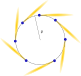
\includegraphics[width=.5\columnwidth]{synchrotron_classical.png}
\caption{Synchrotron radiation.}
\end{figure}


based on Jon Wood and Jackson:
Solving the equations that gives

\begin{equation}
\frac{d^2 I}{d\omega d\Omega} = \frac{e^2}{12 \pi^3 c \epsilon_0} \left(\frac{\omega \rho}{c}\right)^2 (\gamma^{-2} + \theta^2)^2 \left[K_{2/3}^2 (\psi) + \frac{\theta^2}{(1/\gamma^2)+\theta^2}K_{1/3}^2(\psi)\right]
\end{equation}

\begin{equation}
\psi = \frac{\omega \rho}{3c} \left(\frac{1}{\gamma^2} + \theta^2\right)^{3/2}
\end{equation}

\begin{figure}
\centering
\includegraphics[width=.5\columnwidth]{synchrotron_onaxis.png}\includegraphics[width=.5\columnwidth]{synchrotron_offaxis.png}
\caption{Synchrotron radiation.}
\end{figure}


Critical frequency
\begin{equation}
\omega_c = \frac{3}{2} \gamma^3 \frac{c}{\rho}
\end{equation}
\EliasComm{energy loss per turn.}
\EliasComm{sketch on emission and cones.}

Spectrum (angularly integrated)

\begin{equation}
\frac{dI}{d\omega} = \frac{\sqrt{3}}{4} \frac{e^2}{\pi c \epsilon_0} \gamma \frac{\omega}{\omega_c} \int_{\omega/\omega_c}^{\inf} K_{5/3}(x)dx
\end{equation}

Equation for on- and off-axis synchrotron

\begin{equation}
\frac{d^2 I}{dEd\Omega} = \frac{3e^2}{16\pi^3 \hbar c \epsilon_0} \gamma^2 \frac{E^2}{E_c^2} (1+\gamma^2 \theta^2)^2 [K_{2/3}^2(\psi) + \frac{\gamma^2 \theta^2}{1+\gamma^2 \theta^2} K_{1/3}^2 (\psi)]
\end{equation}

\begin{equation}
\psi = \frac{E}{2E_c}(1+\gamma^2 \theta^2)^{3/2}
\end{equation}

\subsection{Undulator and Wiggler Radiation}

\begin{figure}
\centering
\includegraphics[width=.5\columnwidth]{wiggler_offaxis.png}
\caption{Synchrotron radiation.}
\end{figure}

To harvest and direct the radiation of an accelerated relativistic electron more efficiently a set of alternating magnets is used. The electron oscillates and emits radiation preferentially at the turning points as the acceleration is the strongest there and in a forwards-pointing cone with a diameter proportional to $1/\gamma$.

The rapid change of direction in the field and hence forced trajectory of the electron in transversal direction results in a change of effective Lorentz factor in the forward direction.

\begin{equation}
\left\langle\gamma\right\rangle \approx \frac{\gamma}{\sqrt{1 + 0.5 K^2}}
\end{equation}

Commonly two regimes are identified based on the wiggler parameter:

\begin{equation}
K = \frac{eB_0}{m_e ck_u} = \frac{e B_0 \lambda_u}{2\pi m_e c}
\end{equation}

For $K \ll 1$ it is called undulator regime, large $K \gg 1$ indicate the wiggler regime.
In the wiggler regime the divergence of the cone is larger and the radiation has a large bandwidth.
In the undulator regime the radiation is strongly collimated and interference can occur resulting in single harmonics being emitted.

Constructive interference with harmonics of wavelength:

\begin{equation}
\lambda = \frac{\lambda_u}{2 n \gamma^2} \left( 1+ \frac{K^2}{2} + \gamma^2 \theta^2\right)
\end{equation}

If an electron beam of sufficient quality is inserted in a very long undulator the emitted radiation and the electron beam are able to interact and modulate resulting in the emission of coherent radiation. This is observed in free-electron lasers.

The equations introduced for synchrotron radiation work similarly for wiggler radiation. The reference to the bending radius is usually replaced by an expression including the magnet periodicity or the $K$ parameter.


For a wiggler this becomes:
\begin{equation}
\omega_c \sim \frac{3}{2} \gamma^2 K k_u c
\end{equation}

\EliasComm{Include explicit equations here.}


\subsection{Betatron Radiation}

Just as the evacuated `bubble' in a wakefield accelerates particles in a similar way as conventional RF cavities would, the generation of X-rays draws another parallel in conventional devices.
\vspace{\baselineskip}

Due to initial transverse momentum on injection, and the focusing and defocusing fields of the cavity, electrons start to oscillate around the central axis. 
The electrons oscillate at the so-called betatron frequency $\omega_\beta$
\begin{equation}
\omega_\beta = \omega_p / \sqrt{2 \gamma},
\end{equation}
which depends on the plasma frequency $\omega_p$ and the energy of the electrons here given by the relativistic Lorentz factor $\gamma$.

\EliasComm{done this derivation earlier and might want to combine sections.}
\EliasComm{add plot to show particle motion either pic or PIC.}

Similarly to electrons in an insertion device (undulator or wiggler) these oscillations lead to the emission of radiation in a narrow forward pointing cone due to the relativistic forward momentum of the particles.
Not surprisingly, the equations describing both processes are very similar.

The collimation depends on $K$, the wiggler parameter (for insertion devices) or betatron strength parameter
\begin{equation}
K = \gamma k_\beta r_\beta,
\end{equation}
where $k_\beta = \omega_\beta / c$ is the wavenumber and $r_\beta$ is the betatron radius, the amplitude of the oscillations. If $K \gg 1$ it is called the undulator parameter.

The radiation generated follows the on-axis synchrotron radiation with a critical energy
\begin{equation}
\boxed{E_c = \frac{3}{4} \hbar \gamma^2 \omega^2_p r_\beta / c,}
\end{equation}
where this energy parameter indicates when approximately half the energy radiated above and below this value.
\vspace{\baselineskip}

The oscillation of the particles and hence the emission of radiation can be enhanced in wakefield experiments by tailoring the wavefront \cite{Mangles2009} or by using different injection mechanisms.
In LWFA betatron radiation typically reaches the soft X-ray regime of a few to tens of keV.

Difference here is that we use an quasi-electrostatic field instead of a magnetic field, but radiation from a synchrotron, an insertion device (wiggler) and betatron radiation share a common description rooted in the equation of motion (figure-of-eight motion) even though using different field structures and $K$ parameters.

\EliasComm{Include some synchrotron equations}

\EliasComm{Include an image of betatron oscillations.}

\EliasComm{Include plots on spectrum on- and off-axis.}


\EliasComm{See O. Pike thesis \cite{PikeThesis}.}

\subsection{Bremsstrahlung}

\begin{equation}
Z + e^- \longrightarrow Z + e^- + \gamma.
\end{equation}

Charged particles that ... atomic collisions... are being accelerated and radiate.
The radiation emitted is commonly called by its German name `bremsstrahlung', which translates into `braking radiation'.

Also sometimes treated as Compton scattering with a virtual photon (from field of the nucleus).

The process of bremsstrahlung is of interest in this context in two ways:
Firstly, we use the process to generate high-energetic gamma radiation. Relativistic electrons accelerated in a laser wakefield accelerator are collided with a high-Z material to convert efficiently into a collimated burst of X-rays.


\begin{figure}
\includegraphics[width=.5\columnwidth]{feyn_brems.pdf}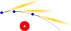
\includegraphics[width=0.5\columnwidth]{brems_classical.png} 
\caption{Classical and feynman diagram.}
\end{figure}

Secondly, the generation of radiation from electrons interacting with solids is an ubiquitous source of noise in the experiments described later on.

Differential cross section under Born approximation (see Jackson):

\begin{equation}
\frac{d \sigma}{d (\hbar \omega)} \approx \frac{Z^2 e^6}{12 \hbar \pi^3 \epsilon_0^3 M^2 c^3} \left(1- \frac{\hbar \omega}{E} + \frac{3}{4} \frac{(\hbar \omega)^2}{E^2}\right) \times \left[\ln\left(\frac{2 E (E-\hbar\omega)}{Mc^2\hbar \omega}\right) - \frac{1}{2}\right] \frac{1}{\hbar \omega},
\end{equation}
for $\hbar \omega < E$.

The number of photons hence scales quadratically with the $Z$ of the converter target used. Higher yield however comes at the cost of spatial resolution and a wider cone of radiation due to scattering in the material. There is a term proportional to $Z$ from electron-electron bremsstrahlung or in other words electrons from the beam interacting with the Z shell electrons of the atom. As the nucleus-electron interaction scales with $Z^2$ is becomes negligible for high-Z materials.

For $\hbar \omega << E$

\begin{equation}
\frac{d^2 \chi_R}{d \omega d \Omega_\gamma} = \left[\frac{3}{2 \pi} \gamma^2 \frac{(1+\gamma^4 \theta^4)}{(1+\gamma^2 \theta^2)^4}\right] \cdot \frac{d \chi_R}{d \omega}
\end{equation}

This means that for highly relativistic electron the emitted radiation is emitted in a narrow forwards-pointing cone. The energy of the emitted radiation is cut off at the energy of the electron.

Bremsstrahlung from relativistic electrons are hence a decent source of broadband high energy gamma radiation.

\EliasComm{Add an explicit plot of the spectrum}
\subsection{Compton Scattering}

Classical Compton scattering describes the inelastic scattering of a photon off an electron which is at rest or close to it. Here the photon loses energy to the electron, hence this is called inelastic. In some conventions this interaction might still be referred to as elastic as energy is transferred into kinetic energy from one particle to another and is not dissipated in terms of heat or deformation. The fully elastic process in the low energy limit is Thomson scattering where the incoming photon does not lose any significant amount of energy in the process.

The reaction can be written as follows:

\begin{equation}
\gamma + e^- \longrightarrow \gamma + e^-.
\end{equation}


\begin{figure}[h]
\centering
\includegraphics[width=0.4\columnwidth]{Compton_Feyn1.pdf}\includegraphics[width=0.4\columnwidth]{Compton_Feyn2.pdf}
\caption{Feynman diagrams for Compton scattering. Time axis from left to right. s- and u-channel.}
\end{figure}

\subsubsection{Kinematics}

\EliasComm{Add a kinematics diagram}

We will treat the electron and the incoming photon both as particles and calculate their final momenta based on energy and momentum conservation in a relativistic framework.
\vspace{\baselineskip}

The electron has a negligible initial momentum $\mathbf{p}_{e,i} = \mathbf{0}$ and the total energy hence reduces to the rest energy of the electron $E_{e,i} = m_e c^2$. The subscript $e$ stands for `electron' and $i$ for initial.
The photon on the other hand has initally a momentum $\mathbf{p}_{\gamma, i}$ and an energy $E_{\gamma, i} = p_{\gamma, i} c = hf$, where $h$ is Planck's constant and $f$ the frequency of the photon. The subscript $\gamma$ represents the photon in this interaction.

Relying on the conservation of energy we can postulate that the sum of energies before and after the interaction have to be equal:
\begin{align}
E_{e, i} + E_{\gamma,i} &= E_{e,f} + E_{\gamma,f},\nonumber\\ 
m_e c^2 + h f &= \sqrt{(p_{e,f} c)^2 + (m_e c^2)^2} + h f',\nonumber\\
hf - hf' +m_e c^2 &= \sqrt{(p_{e,f} c)^2 + (m_e c^2)^2},\nonumber\\
\left( hf - hf' +m_e c^2\right)^2 -(m_e c^2)^2 &= (p_{e,f} c)^2, \nonumber\\
(E_{\gamma, i} - E_{\gamma, f} + m_e c^2)^2 - (m_e c^2)^2 &= (p_{e, f} c)^2.
\end{align}
Here the frequency $f'$ refers to the new frequency of the photon after the interaction.

Similarly we can use momentum conservation to find an expression for the momentum of the electron after the scattering process:
\begin{align}
p_{\gamma, i} &= p_{e, f} + p_{\gamma, f}\nonumber\\
p_{\gamma, i} - p_{\gamma, } &= p_{e, f}\nonumber\\
(p_{\gamma, i} - p_{\gamma, f})^2 &= (p_{e, f} )^2\nonumber\\
(p_{\gamma, i}c)^2 + (p_{\gamma, f}c)^2 - 2 p_{\gamma, i}p_{\gamma, f}c^2\cos(\theta) &= (p_{e, f} c )^2,\nonumber\\
E_{\gamma, i}^2 + E_{\gamma, f} - 2 E_{\gamma, i} E_{\gamma, f} \cos\theta &= (p_{e, f} c)^2.
\end{align}

Setting both equations equal we find the familiar equation for the angular dependent change in wavelength of a photon performing Compton scattering with an electron:

\begin{equation}
\lambda_{final} - \lambda_{initial} = \frac{h}{m_e c} (1 - \cos(\theta)) = \lambda_C (1-\cos(\theta)),
\end{equation}
where $\lambda_C = hm_e c$ is the Compton wavelength.

Similarly there is an equation for the emission angle of the electron:
\begin{equation}
\cot(\phi) = \left(1+\frac{hf}{m_e c^2}\right) \tan(\theta/2).
\end{equation}

In terms of photon energy we can write
\begin{equation}
\boxed{E_{\gamma,f} = \frac{E_{\gamma,i}}{1+\frac{E_{\gamma,i}}{m_e c^2}(1-\cos(\theta))}}
\end{equation}


These equations describe an angular dependent energy distribution, but not the probability of those interactions.
For this purpose we require the differential cross section for Compton scattering.

\subsubsection{Cross-Section}


\begin{figure}
\centering
\includegraphics[width=.5\columnwidth]{Compton_kinematic.pdf}\includegraphics[width=.5\columnwidth]{Compton_KN_cross.pdf}
\caption{Kinematics and differential cross section for different photon energies. The electron is at rest.}
\end{figure}


The cross section combines the kinematics of the process (as discussed) with the matrix element of the interaction which includes the physics of the interaction.

This derivation is based on Peskin and Schroeder \cite{PeskinSchroeder} and Schwartz \cite{Schwartz}.

\EliasComm{add visualisation for ICS (own)}

The spin-averaged Klein-Nishina formula:
\begin{equation}
\frac{\mathrm{d}\sigma}{\mathrm{d}\cos{\theta}} = \frac{\pi \alpha^2}{m^2}\left(\frac{\omega'}{\omega}\right)^2 \left(\frac{\omega'}{\omega} + \frac{\omega}{\omega'}-\sin^2{\theta}\right).
\end{equation}


\begin{equation}
\frac{d \sigma}{d \Omega} = \frac{3}{16 \pi} \sigma_T \left(\frac{E_f}{E_i}\right)^2 \left(\frac{E_i}{E_f} + \frac{E_f}{E_i} - \sin^2 \theta \right)
\end{equation}

For very low energetic photons in the limit $\omega \rightarrow 0$ the cross section simplifies to 
\begin{equation}
\frac{\mathrm{d}\sigma}{\mathrm{d}\cos{\theta}} = \frac{\pi \alpha^2}{m^2} (1 + \cos^2\theta),
\end{equation}
with a total cross section of $\sigma_{total} = 8\pi\alpha^2/(3m^2)$. This is the Thomson scattering cross section.

This cross section and kinematics holds for an electron at rest and a single photon. The cases of one or multiple photons interacting with a relativistic electron are discussed in the following section.

The emission spectrum of Compton scattering at low photon energies is symmetric in the forwards and backwards direction. At increasing photon energies reaching the X-ray and gamma regime the photon is preferentially scattered in the forwards direction.

\EliasComm{Add a low energy differential cross section and spectrum here.}

\subsection{Linear Inverse Compton Scattering}

Laser wiggler. Electric field component, later on at high intensities the magnetic field becomes important as well.

\begin{figure}
\centering
\includegraphics[width=0.8\columnwidth]{ICS_Jason.png}
\caption{Visualisation of inverse Compton scattering (ICS). A relativistic electron is counter-propagated with a laser pulse which gains energy from the interaction due to the relativistic Doppler-effect. Graphics by Jason Cole (Imperial College). REPLACE VISUALISATION BY OWN.}
\end{figure}

\EliasComm{need new ICS visualisation.}

In inverse Compton scattering (ICS) a relativistic electron scatters with one (linear ICS) or multiple photons (non-linear ICS). Whilst in Compton scattering (CS)  momentum is transferred from the photon to the electron (heating), resulting in a longer wavelength of the scattered photon, in ICS the photon gains energy (hence inverse Compton scattering) as it experiences a relativistic Doppler shift. In a different picture this is again a wiggler, this time a laser wiggler making the electrons oscillate with a $K$ parameter of the normalised vector potential $a_0$. In the linear regime this value is $a_0 < 1$ and hence harmonics are emitted similarly as in an undulator.

The photon energies accessible with sufficiently relativistic particles is multiple orders of magnitude higher. In all optical Compton sources \cite{TaPhuoc2012_ICS} relativistic electrons of several hundreds of $\mathrm{MeV}$ have been collided with high-intensity laser pulses, producing tunable X-rays in the $\mathrm{keV}$ \cite{TaPhuoc2012_ICS,Powers2014_ICS,Khrennikov2015_ICS} to $\mathrm{MeV}$ \cite{Chen2013_ICS,Sarri2014_ICS} range with pulse durations of the order of tens of femtoseconds and a micron-scale source size.

In addition to all-optical schemes, it has also been proposed to combine conventional accelerator elements with high-intensity lasers to reach high stability and repetition rates\cite{Seryi2015}.
\vspace{\baselineskip}

The results of a ICS experiment via LWFA at the Astra Gemini facility in the UK are presented later in this report. 

ICS has been widely used in the conventional accelerator community to measure the spin-polarisation of beams.

\subsubsection{Kinematics}

To calculate energy distribution, we can treat this scattering process similarly to the standard Compton scattering we discussed. This requires shifting frames of reference. In the lab frame $S$ quantities will be denoted as before $E, \theta$ and so on. In the rest frame of the electron $S'$ quantities will be denoted as such $E', \theta'$ and so on.

Assume a single relativistic electron beam with a gamma factor $\gamma$ moving in x and a photon of energy $E_{i}$ with an incident angle $\theta_i$.
In the rest frame of the electron the photon experiences a relativistic Doppler-shift. 

\begin{equation}
E'_i = \gamma E_i (1-\mathbf{\beta} \cdot \mathbf{e_k}) = \gamma E_i (1 - \beta \cos\theta) \approx \gamma E_i (1- \cos\theta),
\end{equation}
where we assumed that the electrons are highly relativistic and $\beta \approx 1$.
In a head-on collision ($\theta = \pi$) the photon energy is in the electron rest frame by a factor $2\gamma$ higher.
For $E'_i << m_e c^2$ we are now in the Thomson scattering regime in this frame of reference.

In the rest frame we can now treat this normally for Compton scattering. The photon energies of the scattered photon and the angles follow the previously discussed equations.

\begin{equation}
E'_f = \frac{E'_i}{1+\frac{E'_i}{m_e c^2}(1-\cos\alpha')},
\end{equation}
where $\alpha'$ is the difference between the incident and outgoing angle. As for normal Compton scattering the photon is now losing energy in this frame.

\begin{figure}
\centering
\includegraphics[width=0.8\columnwidth]{boost_temp.png}
\caption{Boost and reference frames.}
\end{figure}
\EliasComm{Make own illustration of kinematics and boosted frame. (This is a screenshot from some slides, will make own illustration)}

\begin{equation}
\cos \alpha' = \mathbf{n'_f} \cdot \mathbf{n'_i} = \cos \theta'_i \cos \theta'_f + \sin \theta'_i \sin \theta'_f \cos(\phi'_i - \phi'_f)
\end{equation}
with $\phi'$ angles being the azimuthal angles of the photon.

The energies have to be boosted back into the lab frame. This gives another factor amplifying the energy of the photon
\begin{equation}
E_f = E'_f \gamma (1+\beta \cos \theta'_f) \approx E'_f \gamma (1+ \cos \theta'_f)
\end{equation}

From these equations we see that the maximum energy can be achieved in a head-on collision and observing the radiation on-axis.
The photons are boosted by $(2\gamma)^2$ to an energy $E_{f,max} = 2 \gamma E'_f = 2 \gamma E'_i = 4 \gamma^2 E_i$.


\subsubsection{Cross-Section}

The calculation of the cross section follows the same scheme, relying on the quantum-corrected Klein-Nishina equation using the angles and energies in the electron rest frame. The angles corresponding to the cross sections and the solid angles, however, have to be transformed in a similar way.

At $\gamma \gg 1$ we will assume that the collisions are always head-on, such that $\sigma' = \sigma$ and we need to only change the solid angle.
Due to the relativistic boost the energy of the photons will look as if $2\gamma$ higher and we will be in the regime where the Klein-Nishina equation already indicates a headlight effect of the radiation being preferably emitted in forwards direction.



\EliasComm{add plot for relativistic kinematics.}
\EliasComm{at $a_0 < 1$ but close to 1 already higher harmonics etc., so not purely first order.}

\subsection{Nonlinear Inverse Compton Scattering}

In nonlinear ICS the $a_0$ of the laser pulse is larger than unity. On the microscopic level this allows for several photons to interact with one electron at a time resulting in higher harmonics being emitted. In a classical picture the electrons perform a figure-of-eight motion due to the intense laser pulse which gives rise to harmonics. This is another parallel to the description of electrons in insertion devices. Similarly as when moving from the undulator regime with distinct harmonics to the wiggler regime with large bandwidth, here also the $K$ parameter linked to $a_0$ increases and rapidly gives rise to hundreds of harmonics forming a smooth synchrotron-like radiation spectrum.

\begin{equation}
n\gamma_L + e^- \longrightarrow \gamma + e^-.
\end{equation}

\begin{figure}
\centering
\includegraphics[width=.9\columnwidth]{feyn_nICS.pdf}
\caption{Feynman diagram for Volkov state equivalent to infinite series of diagrams}
\end{figure}

\subsubsection{Kinematics}

Relativistic kinematics is identical for one or several photons as many incoming identical energy photons and one outgoing with n times $\omega$ the energy. When following the kinematics through one arrives at the same equation as previously for the scattering process in the rest frame of the electron

\begin{equation}
E'_f = \frac{n E'_i}{1+\frac{n E'_i}{m_e c^2}(1-\cos\alpha')},
\end{equation}

At laser intensities reaching an relativistic regime $a_0 \sim 0.1$ the equation of motion of the electron starts deviating from a simple up-and-down oscillation due to a longitudinal component. The electrons start performing a figure-of-eight motion with a longitudinal component increasing with $a_0$.
This additional component has two effects:
Firstly, the modification of the equation of motion leads to a redshifting of the spectrum. The energy of the Doppler-shifted radiation is damped to 
\begin{equation}
\hbar \omega' \approx \frac{4 \hbar \omega a_0 \gamma^2}{1+a_0^2/2 + \gamma^2 \theta^2},
\end{equation}
This leads to a downshift and broadening of the radiation.

We solved the equation of motion previously and it follows the relativistic Doppler shift.

\begin{equation}
\omega' = \gamma \omega (1-\beta \cos(\theta)) \approx \omega (1+\gamma^2 \theta^2)/2\gamma
\end{equation}

Secondly, energy is being transferred from this fundamental radiation at $\omega$ to higher order harmonics $\omega_1 = n\omega$, when multiple photons upconvert to one higher energy photon. Since this is a free electron process the harmonics are not restricted to either odd or even numbers but cover both. Classically, the radiation pattern is calculated using Fourier analysis.

The angular distribution of each component is distinct and symmetric, with odd harmonics showing a maximum on-axis and (n-1)/2 lobes on either side and even harmonics having a minimum on-axis and n/2 side-maxima on either side.

\begin{figure}
\centering
\includegraphics[width=.5\columnwidth]{ICS_Redshift.png}\includegraphics[width=.5\columnwidth]{ICS_Redshift2.png}
\caption{Redshift of the fundamental harmonic.}
\end{figure}

\EliasComm{make a plot for the spectrum and correct this spectrum to reflect the spectrum in the lab frame or make notable that this is in the rest frame. Maybe compare the two.}

In the highly nonlinear regime $a_0 \gg 1$ the number of harmonics increases by a factor $a_0^3$ (REF ESAREY RIDE SPRANGLE PRE 1993) $n_c \approx 3 a^3_0/4$. At the same time each harmonic is spread out due to the longitudinal component which now dominates the electron motion.

The high number of harmonics (hundreds!) and the redshifting of each component transforms the spectrally very peaked spectrum to a broadband source resembling a synchrotron spectrum.

This means to reach higher photon energies a more intense laser is not necessarily the best option as the redshifting appears rapidly along with the harmonics. A more energetic electron provides a redshift-free upshift. If one wants a close to monoenergetic spectrum on top of that linear Compton scattering in the limit $a_0 \rightarrow 0$ is more suitable.

\subsubsection{Cross-Section}

Volkov state, Furry picture, dressed states.

Infinite series of diagrams in this set.

\EliasComm{One, two photon feynman diagrams. Add image of dressed states and series equivalent.}

Models: classical harmonics, polarisation dependency, quantum model.

\EliasComm{See Naroshny 1965 Soviet JETP, KT McDonal 1986, dsigma/dx = ... Jl(x)/(1+x)2}

In the classical derivation this becomes a Fourier analysis and the electron trajectories (see figure of eight motion) leads to higher harmonic generation.
The emission spectrum is composed of generalised Bessel functions.

\begin{equation}
\sim \Sigma ... C_x^2(1-\sin^2\theta\cos^2\phi)+C_z^2\sin^2\theta-C_x C_z \sin2\theta\cos\phi
\end{equation}

\begin{equation}
C_x = \Sigma (-1)^m j_m(\alpha_z) (J_{n-2m-1)} ...)
\end{equation}

Use some Bessel identities (see appendix) and $\theta = 0$. (There are also small angle solutions I believe).

The specific case of on-axis backscattering leads to the differential expression (REF Esarey):

\begin{equation}
\sim n \alpha_n \left[ J_{(n-1)/2}(\alpha_n) - J_{(n+1)/2}(\alpha_n)\right]^2
\end{equation}

For odd harmonics. For even harmonics the generalised Bessel function vanishes. This means there are only odd harmonics on the axis. However, there are off-axis contributions with both harmonics and very close at higher orders.

\subsubsection{Other modifications of the spectrum}

In a real setting the ICS spectrum is modified by several input parameters:
the energy spread of the electron beam will translate to an energy spread in the ICS spectrum.
Short pulse lasers intrinsically require a certain bandwidth are hence not monochromatic. The spread of photon energies modifies the spectrum similarly.
Deviations from a head-on collision have to be considered and also introduce a spread, in particular considering divergence and emittance of the electron beam and the range of angles of the focusing laser pulse with respect to the laser axis.


\section{Radiation Reaction}

The previous sections left out the effect of radiation losses onto the equation of motion of charged particles.
Charged particles emit radiation when being accelerated. The charged particle emitting the radiation loses the energy associated with the photon and is knocked back, adhering to momentum and energy conservation rules. This is called radiation reaction (RR) or radiation friction.
Radiation reaction is a very fundamental problem of physics, but surprisingly a universally accepted description does not exist thus far (REF). Each description only exists in a certain limit and is an approximation valid within those limits, but breaks down in extreme conditions (REF). High field QED is a suitable environment to test the limits of these models (REF).
\vspace{\baselineskip}

Whilst the emission of radiation is ubiquitous, in many cases radiation losses are small or occur over longer spans of time which means they can be ignored or the detailed physics of radiation reaction is not important. In storage rings of large accelerator and collider facilities radiation losses pose a significant problem as they limit the maximum energy the particles can be accelerated to. The exact dynamics of radiation reaction and the influence on the equation of motion of the particles is not very significant. It suffices to add the average energy lost over the a turn in the storage ring to prop up the system. This is sometimes referred to as weak radiation reaction (REF).

Radiation reaction effects become more significant in extreme conditions where ultra-relativistic particles interact with light: in astrophysical phenomena relativistic particle jets of GeV, TeV or PeV level are frequently observed. Interacting with the ubiquitous CMB inverse Compton scattering provides a high energy background radiation (REF).
These conditions are re-constructed in laser and accelerator facilities interacting ultra-relativistic particles with laser pulses. Radiation reaction was measured, for instance, at SLAC \cite{Bula1996_RR,Burke1997_RR}, and at the LHC \cite{Wistisen2018_RR} and first measurements have been undertaken at non-conventional accelerators such as the Astra-Gemini laser system at the Central Laser Facility in the UK \cite{Cole2018_RR,Poder2018_RR}. This work is part of this thesis (see Chapter \ref{Chap:RR15}, \nameref{Chap:RR15}).
\vspace{\baselineskip}

In this section a selection of radiation reaction models are motivated and introduced. Since this is a fundamental problem a variety of different approaches have been tried, but the author will restrict this section to the most commonly discussed models which are also relevant to this work.

Firstly, the first intuitive approach to radiation reaction is explored: simply adding an external force $m \ddot{x}$ to the equation of motion. In covariant form this is the Lorentz-Abraham-Dirac force or short LAD. This set of solutions results in pathological solutions or so-called runaway solutions with self-acceleration and unphysically requiring knowledge of the future.

Secondly, a first self-consistent solution is presented: the Landau-Lifschitz model (LL). This model does not have pathological runaway solutions and employs retarded potentials resulting in the right causality. The Landau-Lifschitz model is a perturbation model for $F_{RR} \ll F_{Lorentz}$ and hence is valid only within this limit. For large RR forces the LL model gives rise to unphysical solutions, in particular it predicts the emission of radiation greater than its own total energy.

After discussing these classical approaches to radiation reaction, finally, a model based on a quantum picture is introduced. Here an electron passing through a high intensity field can either be described by a series of individual multi-photon Feynman diagrams or as an electron in a dressed state, the Furry picture. The latter is appropriate in the context of high-field QED. We find that the quantum picture provides two important corrections to the classical picture: one is the adjustment of the radiation spectrum and power eliminating the unphysical emission of radiation larger than the electron energy by introducing a cut-off. This reduction of emitted power can be parametrised by the Gaunt factor and applied to the LL model as a continuation into the high-field regime, resulting in a semi-classical model with classical equations of motion but an emission power adjusted to the quantum picture. The other adjustment is the introduction of stochasticity. The quantum world is inherently non-deterministic and bound to probabilities. One initial state does not always end up in the same final state even if the boundary conditions are identical. This results in interesting phenomena including a hardening of the photon spectrum and a widening of the electron energy spread.

However, even the model presented is derived within a framework relying on approximations. In this case this is the local constant field approximation (LCFA) which assumes that during the formation time of the photon the electric field does not change significantly. For an extremely intense oscillating electromagnetic field, for instance an intense laser field, this might not always be true and even this model might have its limitations. The LCFA is introduced and its potential limitations are shown as motivation for future research.

\subsection{Radiation reaction: classical runaway solutions}

This section is based on Jackson. \cite{Jackson}
One intuitive way to derive an expression for radiation reaction is considering conservation of energy. It is well known that accelerated charges emit radiation which is fairly well characterised in the context of synchrotrons, other circular accelerators or undulator setups. The emitted power follows the Larmor power formula

\begin{equation}
P = \frac{2}{3} \frac{e^2}{c^3} \mathbf{\dot{v}}^2.
\end{equation}

This equation can be used to derive an expression for a radiation force by integration.
The explicit steps can be found in Jackson (Chapter 16, equations 16.7 to 16.8).

The in Jackson called `radiative reaction force' then becomes
\begin{equation}
F_{rad} = \frac{2}{3} \frac{e^2}{c^3}\mathbf{\ddot{v}} = m \tau \mathbf{\ddot{v}}.
\end{equation}

The equation of motion then reads
\begin{equation}
m(\mathbf{\dot{v}}-\tau \mathbf{\ddot{v}}) = \mathbf{F}_{ext}.
\end{equation}

This equation of motion, sometimes referred to as Abraham-Lorentz equation, depends on the second derivative of the velocity in time which results in runaway solutions.
For a vanishing external force, we obtain two solutions for $\mathbf{\dot{v}}$:
\begin{equation}
\mathbf{\dot{v}}(t) = 0 \,or\, \mathbf{a}e^{t/\tau}.
\end{equation}

$\mathbf{a}$ is the acceleration at $t = 0$. If $\mathbf{a} \neq 0$ we run into trouble.

First attempts to simply add radiation reaction as a force onto the Lorentz-force equation resulted in unphysical expressions depending on several derivatives of the velocity. This in the end required knowing about the future to calculate its equation of motion, and led to self-acceleration of the particles in question. These solutions are commonly referred to as `runaway solutions'.

The relativistic generalisation was found by Dirac renormalising in 4-space. The result is referred to as Lorentz-Abraham-Dirac equation (LAD).


\EliasComm{Jackson seems to be in cgs. Make sure you know which unit system you work in.}

\EliasComm{Despite the runaway solution: if one ignores this solution tree, are the predictions feasible?}

\subsection{Self-consistent classical description: Landau-Lifschitz}

A first self-consistent solution to including radiation reaction into a classical model was achieved by Landau and Lifschitz (REF).
LL solution is a perturbation and means the radiation reaction force has to be small compared to the Lorentz force and a suitable frame of reference has to be found to make this valid. In some cases energy conservation might be violated in an abruptly changing EM field.

Problems: energy loss can exceed initial energy. Stochasticity not included.

In EM four vector form \cite{Bulanov2011_LADLL}:

\begin{equation}
g^\mu = \frac{2e^3}{3m_e c^3} \left\lbrace   \frac{\partial F^{\mu \nu}}{\partial x^\lambda} u_\nu u_\lambda - \frac{e}{m_e c^2} \left[ F^{\mu \lambda} F_{\nu \lambda} u^\nu - \left(F_{\nu\lambda}u^\lambda\right) \left( F^{\nu\kappa}u_\kappa\right)u^\mu \right]   \right\rbrace
\end{equation}

In 3-dim.

\begin{equation}
\mathbf{F} = \frac{2e^3}{3m_e c^3 \sqrt{1-\frac{v^2}{c^2}}} \left\lbrace \left( \frac{\partial}{\partial t} + (\mathbf{v} \cdot \nabla) \right) \mathbf{E} + \frac{1}{c} \left[ \mathbf{v} \times \left( \frac{\partial}{\partial t} + (\mathbf{v} \cdot \nabla) \right) \mathbf{B} \right] \right\rbrace +\\
+ \frac{2e^4}{3m^2_e c^4}\left\lbrace \mathbf{E}\times\mathbf{B} + \frac{1}{c} ( \mathbf{B} \times (\mathbf{B} \times \mathbf{v})) + \frac{1}{c} \mathbf{E} (\mathbf{v} \cdot \mathbf{E}) \right\rbrace - \\
- \frac{2e^4}{3m^2_e c^5 \left( 1-\frac{v^2}{c^2}\right)} \mathbf{v} \left\lbrace\left( \mathbf{E} + \frac{1}{c} \mathbf{v} \times \mathbf{B}\right)^2 - \frac{1}{c^2} (\mathbf{v} \cdot \mathbf{E})^2 \right\rbrace
\end{equation}

This is an effective model and the violation of energy conservation is possible.

\subsection{Quantum picture and corrections}
\EliasComm{Furry picture, treating the laser field as classical external field.}

Alec says that quantum radiation reaciton is the overall recoil experienced by an electron undergoing multiple simultaneous incoherent photon emission events.

Limit when quantum effects become more important: energy loss comparable to rest mass of the electron?
This is at the same time also the limit of validity of the LL model, when the force becomes comparable to the Lorentz force.

Quantum parameter eta and chi. $\eta = E_{RF}/E_{crit}$
Critical field for quantum electrodynamics $E_{crit} = 1.38 \times 10^{18}\,\mathrm{V m^{-1}}$
The field in the rest frame becomes important in relation to the critical field. This is somewhat similar to the approximation that the field be much smaller than the Lorentz force.

With high confidence we know that we require a quantum description of this process.
There are several ways to solve some of the issues of the classical Landau-Lifschitz description.

Estimate relative magnitude (LL)

\begin{equation}
\psi = \gamma^2 a_0 \frac{2 r_e \omega}{3c}
\end{equation}

REFS: Chris Ridgers JoP \cite{Ridgers2017_QRR}

Corrections regarding spectrum of radiation (cut-off).

Stochasticity.

Semi-classical approach using Gaunt factor (power!).

\begin{equation}
g(\eta) = \frac{\int_0^{\eta/2} F(\eta, \chi) \mathrm{d}\chi}{\int_0 F_{cl}\left(\frac{4\chi}{3\eta^2}\right)} = \frac{3 \sqrt{3}}{2 \pi \eta^2} \int_0^{\eta/2} F(\eta,\chi) \mathrm{d}\chi. 
\end{equation}

Fit for function is (Baier 1991):

\begin{equation}
g(\eta) \approx \left(1 + 4.8(1+\eta)ln(1+1.7\eta)+2.44\eta^2\right)^{-2/3}.
\end{equation}

Assuming local constant cross field approximation (LCFA).
Formation time, coherence time.
What is the force in this picture? How does it compare to ponderomotive force?

Adjustment of the emission spectrum (comparison)

Adjustment of the electron spectrum in interaction: cooling versus heating term.

Cooling of spectra versus competing processes.

\subsection{Measuring radiation reaction}

Inverse Compton Scattering

Planar channeling in crystals

\section{Pair Production and Annihilation}

Pairs are easily annihilated in radiactive substances for low energy positrons cancelling out with ambient electrons.
At higher energies the cross section decreases.
Add the relation from O. Pike's thesis \cite{PikeThesis} ($\sigma \sim 2 \beta^2 \sigma$ relating annihilation and pair production?

If this process is so simple, how come the inverse process of colliding two photons has been so difficult in experiment?
This section aims to explain how matter annihilates and inversely matter can be created and where the challenges for these methods lie.

\subsection{Pair annihilation}

The annihilation of electron-positron pairs is commonly found in radioactive decays following this simple equation:
\begin{equation}
e^+ + e^- \longrightarrow 2 \gamma.
\end{equation}
Matter and antimatter meet and annihilate into pure energy converting the rest mass of both particles into photons. In radioactive decays relatively slow pairs collide and the emitted gamma rays are coincident emitted at 180 degrees in the centre-of-mass frame. This is used in radio-isotope therapy to localise the tumour.

\subsubsection{Kinematics}
An electron-positron pair at rest, i.e. total momentum was zero before the interaction. This means that the 2 gamma photons will leave (in that frame) back-to-back.
These photons carry away the same energy. Deviations can be found once the electron and positron carry a kinetic energy.

\subsubsection{Cross section}
\begin{equation}
\sigma_{e^+ e^-} = \frac{\pi r^2_e}{2} (1-\beta^2) \left[ (3-\beta^4) ln\left(\frac{1+\beta}{1-\beta}\right) - 2 \beta (2-\beta^2)\right]. 
\end{equation}

\subsection{Bethe Heitler process}

There are different ways to create pairs:
Bethe Heitler: 
Trident: second order diagram. Electron emits a virtual photon which then decays into an electron-positron pair. Could happen in a two-step process of an electron in an external field (laser) performing inverse Compton.
O. Pike:
\begin{equation}
\frac{d \sigma_{\gamma Z}}{dE_+}(\omega,x) = -\frac{1}{\bar x^2}\frac{d\sigma_{eZ}}{d\omega}(-\omega,x)
\end{equation}

\subsection{Trident process}

Multi-step process.

\subsection{Linear Breit Wheeler}


Linear and nonlinear Breit-Wheeler: two or more photons interact to produce one pair.

\begin{figure}[h]
\centering
\includegraphics[width=0.4\columnwidth]{feyn_BW1.pdf}\includegraphics[width=0.4\columnwidth]{feyn_BW2.pdf}
\caption{Feynman diagrams for Breit-Wheeler pair production. Time axis from left to right.}
\end{figure}


Explain why X-ray and Gamma interaction is suitable:
Need to overcome threshold for interaction. Cross section needs to be directed and hence we need one of the photons to be at much higher energy. Beaming!

Annihilation
\begin{equation}
\sigma_{e^+ e^-} = \pi r^2_0 \frac{(1-\beta^2)}{4\beta^2}\left[(3-\beta^4) ln\left(\frac{1+\beta}{1-\beta}\right) - 2 \beta (2-\beta^2)\right]
\end{equation}


Linear Breit Wheeler kinematics



Linear Breit Wheeler cross section

In CM frame, from \cite{Ribeyre2016_BW} (Pair creation in collision of gamma-ray beams produced with high intensity lasers) also found in O. Pike's thesis \cite{PikeThesis}

\begin{equation}
\sigma_{\gamma,\gamma} = \frac{\pi r^2_e}{2}(1-\beta^2) \left[(3-\beta^4) ln\left(\frac{1+\beta}{1-\beta}\right) - 2 \beta (2-\beta^2)\right] = 2 \beta^2 \sigma_{e^+ e^-}
\end{equation}

$s = (E^*/m_e c^2)^2 = E_{\gamma 1} E_{\gamma 2} (1-\cos\phi)/2 m^2_e c^4, \beta = (1-1/s)^{1/2}$

For head-on collision $\theta = \pi \rightarrow s = E_1 E_2/m^2_e c^4$ and for $\theta = \pi/2 \rightarrow s = E_1 E_2/2m^2_e c^4$.
The threshold is $s > 1$.


\subsection{Nonlinear Breit Wheeler}

Nonlinear Breit Wheeler 
Seen at SLAC E144 \cite{Bula1996_RR,Burke1997_RR}

Many photons interacting with one to generate pairs.

\EliasComm{Do not go into detail here as we are not investigating the non-linear process here.}

\subsection{Schwinger limit}

Schwinger pair production: The external electric field is so strong that virtual electron-positron pairs can be accelerated to relativistic energies within a Compton wavelength and made real.

\section{A side note: Other High-field phenomena}

High-field QED is an exciting area of research. Where there is an extremely intense laser pulse exciting physics happens: light becomes matter, the vacuum interacts with the laser and the vacuum gives birth to matter.

\subsection{Photon-Photon scattering}
Discussing high-field phenomena and the limit where pair production becomes feasible a short note on photon-photon scattering appears appropriate.
Where a large density of photons are at the same place, at high intensities, as required for the Schwinger limit, the probability for photons to scatter from other photons becomes significant.

Photons can scatter from other photons mediated by virtual electron-positron pairs. This is not a tree-level diagram but involves at least 4 vertices reducing its probability to virtually zero. At high intensities the coupling increases and these higher order diagrams can contribute significantly.

\subsection{Vacuum birefringence}

An intense laser pulse propagating through vacuum will also experience a modification. As the quantum vacuum is everything but void it also carries a refractive index and birefringence capacities. At the high-field limit these effects are expected to become visible.